\documentclass[figures, tables, times]{outhesis}
% Class options are: master, tables, figures, algorithms, index, times
% and compact

% Use these packages for an English dissertation without the Times font
% \usepackage[latin1]{inputenc}
% \usepackage[T1]{fontenc}
% \usepackage[english]{babel}
% \usepackage{lmodern}

% Insert additional packages and commands below
\usepackage[amssymb]{SIunits}  % allows SI units
\usepackage[pdftex]{graphicx}  % allows .eps and .epsi graphics to be inserted
\usepackage{epic}              % allows use of latex graphics
\usepackage{eepic}             % allows use of latex graphics
\usepackage{varioref}
\usepackage{amssymb,amsmath}   % Amer. Math. Soc. packages
\usepackage{amsfonts}          % Amer. Math. Soc. special fonts package
\usepackage[centerfoot]{pageno} % allows positioning of page numbers
\usepackage{natbib}            % citations with ametsoc.bst
\usepackage[table]{xcolor}     % allow for alternating row colors in table
\usepackage{longtable}
\usepackage{array}
\usepackage{hyperref}
\usepackage[bottom]{footmisc}
\usepackage{multirow}
\labelformat{equation}{\textup{(#1)}}
\labelformat{enumi}{\textup{(#1)}}
\bibpunct{(}{)}{;}{a}{}{,}    % AMS uses ``author year'' not ``author, year''
\IfFileExists{revision.sty}{\usepackage{revision}}{}

% Required commands
\title{A Method for Calibrating Probabilistic Forecasts}
\author{PATRICK TIMOTHY MARSH}
\degreename{DOCTOR of PHILOSOPHY}
\gradyear{2013}
\school{SCHOOL OF METEOROLOGY}
\chair{Dr.~Kevin A.~Kloesel}
\abstractfile{./extras/abstract} % Insert Abstract file name in between brackets
% The commands \abstractfile, \thanksfile and \appendixfile take filenames as
% arguments. The source of the abstract (and the acknowledgements and the
% appendix) must be placed inside a separate file which name is the argument
% of the command \abstractfile (and thanksfile and \appendixfile).

% Optional commands
\cochair{Dr.~John S.~Kain} % Co-chair (if any)
\readerA{Dr.~David J.~Stensrud}
\readerB{Dr.~Michael B.~Richman} % Additional readers (up to four)
\readerC{Dr.~Frederick H.~Carr}
\readerD{Dr.~S.~Lakshmivarahan}
% \dedication{text} % Insert dedication text in between brackets
\thanksfile{./extras/acknowledgements} % Acknowledgments file name goes in between brackets
% \appendixfile{filename} % Insert Appendix file name in between brackets

\begin{document}
\makefrontmatter
\sloppy

% Insert the dissertation text below or the relevant \input command
%!TEX root = ../dissertation.tex


\chapter{Introduction}
\label{intro}

Rare meteorological events\footnote{\cite{Murphy1991} defined a rare meteorological event as one that occurs on less than five percent of forecasting occasions.} that occur on small spatial and short temporal scales pose significant challenges to forecasters.
This is related to the limited predictability of phenomena occurring on short time-space scales; however, these events comprise a substantial portion of meteorological phenomena that negatively impact society (e.g., heavy rain, large hail, tornadoes, etc.).
Thus, ``good'' forecasts of these events would provide large societal benefits.


What makes a ``good'' forecast has been the subject of many discussions throughout the history of forecasting (e.g. \citealp{Peirce1884, Clayton1889, Nichols1890, Mascart1922, Winkler1968, Murphy1993, Murphy1996} and papers therein).
In an essay designed to address this question, \cite{Murphy1993} provided three distinct measures of forecast ``goodness'': consistency, quality, and value.
Consistency, sometimes referred to as \mbox{type 1} ``goodness'', is a measure of correspondence between the actual forecast and the forecaster's judgment of what will occur.
Quality, sometimes referred to as \mbox{type 2} ``goodness'', is a measure of correspondence between the forecast and the observations.
Value, known as \mbox{type 3} ``goodness'', is a measure of the benefit a forecast provides to users of the forecast.


A natural consequence of maximizing consistency is the need for probabilistic forecasts.
This is the result of the uncertainty in a forecaster's judgment that must be conveyed in the resulting forecast.
When forecasters produce probabilistic forecasts that accurately depict their uncertainty, the best expected quality, as measured by a strictly proper scoring rules \citep{Winkler1968}, is also achieved, cementing the need for forecasts to have a probabilistic component.


Prior to the twentieth century, weather forecasts were largely the result of rules of thumb, with little understanding for the physical mechanisms governing the atmosphere.
However, several attempts at utilizing probabilities (and odds) in weather forecasts date back to the late eighteenth century when J. Dalton included measures of uncertainty in his forecasts \citep{Dalton1793, Murphy1998}.
Although the exact forecast methods of Dalton are not known, Dalton's forecasts include statements such as ``the probability of rain was much smaller than at other times'' and ``the probability of a fair day to that of a wet one is as ten to one,'' \citep{Murphy1998}.
Nearly a century later, in 1871, under the direction of Professor Cleveland Abbe, the first forecasts and warnings issued by the United States Signal Service were actually labeled probabilities. \citep{Whitnah1961, Murphy1998}.
In fact, Professor Abbe promoted the use of ``probabilities'' so much he earned the nickname ``Old Probabilities'' \citep{Scott1873, Murphy1998}.


Although probability forecasting of some variety was performed prior to the start of the twentieth century, the start of probability forecasting is often attributed to the work of W. E. Cooke \citep{Murphy1998}.
\cite{Cooke1906a} eloquently summarized the shortcomings of deterministic forecasting, and championed the inclusion of uncertainty information, by stating:
\begin{quote}
    ``(a)ll those whose duty it is to issue regular daily forecasts know that there are times when they feel very confident and other times when they are doubtful as to the coming weather. It seems to me that the condition of confidence or otherwise forms a very important part of the prediction, and ought to find expression. It is not fair to the forecaster that equal weight should be assigned to all his predictions and the usual method tends to retard that public confidence which all practical meteorologists desire to foster. It is more scientific and honest to be allowed occasionally to say `I feel very doubtful about the weather for tomorrow'\dots and it must be\dots useful to the public if one is allowed occasionally to say `It is practically certain that the weather will be so-and-so tomorrow''' (\mbox{p. 23}; \citealp{Murphy1998}).
\end{quote}


\noindent\cite{Cooke1906a} went on to propose a forecasting paradigm in which a forecaster assigned a set of uncertainty weights to each forecast.
The uncertainty weights were designed to express various levels of confidence, and it was shown that forecasters were were able to assign weights that appropriately reflected their uncertainty.
Although these forecasts conveyed uncertainty information, they were not fully probabilistic in nature.
It wasn't until \cite{Hallenbeck1920} that numerical probabilistic forecasts were recorded in the literature.


Around the same time as the work done by Hallenbeck, a series of papers by Anders {{\AA}}ngstr{{\"o}}m poignantly made the case for probabilistic warnings, rather than binary or categorical \citep{Angstrom1919, Angstrom1922, Liljas1994, Murphy1998}.
The crux of {{\AA}}ngstr{{\"o}}m's arguments revolved around the difficulties forecasters face when they are constrained to issue a warning in binary terms.
This difficulty, argued {{\AA}}ngstr{{\"o}}m, arises from the fact that forecasters' knowledge of users' cost/loss ratios is generally insufficient to determine whether to ``issue a warning" or ``not issue a warning" in the context of producing the best possible forecast for users.
{{\AA}}ngstr{{\"o}}m further noted that ``(w)hat makes the matter still more complicated is the fact that\dots [the loss function]\dots has very different values in different cases," \citep{Angstrom1922, Murphy1998}. {{\AA}}ngstr{{\"o}}m ultimately concluded: ``The most appropriate system seems therefore to be to leave to the clients concerned by the warning to form an idea of the ratio [cost-loss ratio]\dots and to issue the warnings in such a form that the larger or smaller probability of the event gets clear from the formulation.
The client may then himself consider if it is worthwhile to make arrangements of protection or to disregard a given warning," \citep{Angstrom1922, Murphy1998}.
In these two short papers, {{\AA}}ngstr{{\"o}}m succinctly argued the case for probability forecasts.
Unfortunately, advancements in probability forecasting lay dormant until mid-century.


In addition to probability forecasting, the start of the twentieth century marked the conception of numerical weather prediction.
In 1901 Professor Abbe proposed that the atmosphere was governed by a set of dynamic and thermodynamic equations, and that these equations could be used to predict future states of the atmosphere \citep{Abbe1901}.
\cite{Bjerknes1904} followed with the recognition that in order to produce forecasts of subsequent states of the atmosphere based on the governing equations:
\begin{enumerate}
    \item One has to know with sufficient accuracy the state of the atmosphere at a given time; and
    \item One has to know with sufficient accuracy the laws according to which one state of the atmosphere develops from another.
\end{enumerate}
Bjerknes recognized that the creation of a sufficiently accurate analysis of the atmosphere is a necessary condition for reliable forecasts of future atmospheric states based on the integration of the governing equations.


Lewis Richardson took up the challenge of weather prediction in the 1910s and went on to produce the first numerical prediction (i.e. one using mathematical equations; \citealp{Lynch2008}).
The forecast took about \mbox{6 weeks} to produce by hand and predicted the change in surface pressure over the course of \mbox{6 hours}.
Although the forecast was a spectacular failure --- predicting a \mbox{145 mb} surface pressure fall when the barometric pressure remained nearly constant --- Richardson considered it ``a fairly correct deduction from a somewhat unnatural initial distribution,'' \citep{Lynch2008}.
Ultimately, Richardson's forecast was doomed from the start, falling victim to Bjerknes' first requirement for successful numerical forecasts: adequate initial conditions.


In the late 1940s, Jule Charney demonstrated that larger-scale atmospheric motions could be sufficiently predicted by advecting the geostrophic vorticity with the geostrophic wind \citep{Charney1947}.
A few years later, Charney, and his team of researchers, went on to produce the first successful numerical weather forecasts produced from a computer \citep{Charney1950}.
Word of this success spread rapidly throughout the meteorological community, and by the mid-1950s short-term operational numerical weather forecasts were being produced in the United States and Sweden \citep{Lewis2005}.
Although operational numerical forecasts began in the mid 1950s, these forecasts were based on the simplified equations formulated by \cite{Charney1947}.
As a result of the simplified equations used in numerical weather forecasts, some meteorologists began to explore statistical methods to correct the numerical output \citep{Gleeson1961}.
Based on the work of \cite{Hinkelmann1951}, operational numerical forecasts began using the primitive equations to produce numerical forecasts in the mid 1960s \citep{Lynch2008}.


Unfortunately, raw deterministic model output (i.e. output that has not been post-processed) is not probabilistic in nature.
Deterministic model output provides a precise answer at every grid point for all output fields.
This is a consequence of the internal numerics of deterministic models; equations are constrained to produce a single value.
However, raw deterministic model output can still be thought of in terms of probabilities.
A single output value can be interpreted as having a probability of 1 that the output value will be observed, and a 0 that any other value will be observed.
Unless the deterministic model is always perfect, the probability that the model's forecast will be correct lies somewhere between \mbox{0 and 1}.


In the 1960s, Edward Lorenz published a series of papers that demonstrated the chaotic nature of the atmosphere \citep{Lorenz1963, Lorenz1965, Lorenz1968}.
Lorenz demonstrated that even small errors in the initial state of the modeled atmosphere --- even those within observational error --- can have large impacts on the resulting numerical forecast.
These errors abound from all aspects of numerical weather prediction, ranging from numerical to observational to the model itself.
Thus, perfect, deterministic, numerical weather predictions are essentially impossible.
Therefore, in order for a numerical weather forecast to satisfy type 2 ``goodness'' they, too, must include a probabilistic component.


Armed with the results of \cite{Lorenz1963, Lorenz1965, Lorenz1968}, alternatives to the deterministic numerical prediction paradigm began to be offered.
\cite{Epstein1969} recognized that the atmosphere could not be completely described with a single numerical forecast due to inherent uncertainty.
\cite{Epstein1969} and \cite{Gleeson1970} each offered ways to produce probability forecasts in which the numerical model output means and variances directly.
Although these methods showed promise, the addition of uncertainty terms proved to be too computationally expensive for operational use at that time.


\cite{Leith1974} offered the first attempt at Monte Carlo forecasting, or ensemble forecasting as it is known today.
Leith suggested that instead of running a single forecast from a single initialization, a collection (ensemble) of forecasts, each with a slightly different initial state, should be produced.
The resulting forecasts could be used to assess the uncertainty of the forecast.
One such method of assessing the uncertainty is to report the fraction of ensemble members that produce a certain forecast divided by the total number of ensemble members.
This results in a probability of occurrence, derived from the collection of numerical forecasts.
As was the case with \cite{Epstein1969} and \cite{Gleeson1970}, even though this approach showed promise, it was too expensive for operational use at that time.
It took nearly two decades worth of computational advancement, but operational ensemble prediction systems because a reality in the early 1990s.


A different approach was put forth by \cite{Glahn1972}.
Instead of adding additional terms to the numerical model, or producing multiple model forecasts each starting with slightly different initial conditions, the idea was to post-process the raw model output by using statistical models.
The statistical models are in essence multi-variate regressions, derived from the three-dimensional numerical output, observations, and the general climatological conditions for specific locations.
These model output statistics, or MOS, account for model-biases as well as local effects that cannot be resolved by the model due to model grid spacing.
Although some MOS products are deterministic in nature (such as the maximum and minimum \mbox{6 hr} temperatures), some products are probabilistic (such as probability of precipitation).
MOS is still used today by the National Weather Service \citep{Allen2001a, Allen2001b, Sfanos2001, Carroll2005, Glahn2009}.


As previously alluded to, during the latter parts of the twentieth century computing power rapidly increased.
This increase offered numerical weather prediction modelers the opportunity to either decrease model grid spacing or transition to ensemble forecasting.
Most operational numerical weather prediction centers argued in favor of decreasing model grid spacing (e.g, \citealp{McPherson1991, WMO1992}).


The choice to embrace higher resolution numerical models resulted in much needed improvements to the models' physics parameterizations.
Additionally, improved model grid spacing allowed for numerical models to better represent atmospheric phenomenon with strong gradients (i.e., fronts, drylines, inversions, etc.).
These improvements allowed for intoxicatingly detailed forecasts.
When the details of the numerical forecast were correct, highly specific spatial and temporal forecasts were easily produced \citep{Droegemeier1990}.
Unfortunately, the details of numerical weather prediction models are best in environments in which the atmosphere is dominated by large-scale phenomenon (i.e., when quasi-geostrophy can be assumed; \citealp{Antolik1989}).
Thus, numerical guidance tends to be at its best when the forecasting situation is, in some sense, the easiest, and is least needed \citep{Brooks1993}.


Some in the meteorological community, however, argued for adopting ensemble forecasting (e.g. \citealp{Brooks1992a, Brooks1993}).
As previously noted, \cite{Lorenz1963, Lorenz1965, Lorenz1968} demonstrated that a numerical weather forecast was sensitive to the initial conditions.
Unfortunately, model grid spacing is typically less than that at which we observe the atmosphere over the globe.
Thus, in addition to the errors introduced by the observing instruments, additional errors can be introduced as a result of interpolating observations to grid points that do not have collocated observations.
A consequence of this is that the true state of the atmosphere is rarely, if ever, known.


Numerical weather prediction, and in particular, high-resolution models of thunderstorms, has been shown to be very sensitive to small changes in the initial conditions \citep{Lorenz1963, Lorenz1965, Lorenz1968, Brooks1992a, Brooks1992b}.
As a result, the inherent uncertainty in the observations could result in major errors in a forecast from models on that scale.
An ensemble approach recognizes the uncertainty in the initial conditions and utilizes it to produce a collection of forecasts, rather than assuming that the initialization is correct \citep{Brooks1992a}.


History has shown that a compromise of both of the increased resolution and ensemble forecasting paradigms have prevailed.
Operational centers in the United States currently run a global ensemble at relatively coarse resolution, whereas a suite of limited area models are run at increasingly higher resolution as the domain size decreases.
Recently, the computational power has increased to the point of allowing operational limited area model forecasts at grid spacings small enough for the cumulus parameterization scheme to be turned off.
Even with the sensitivities to initial conditions previously mentioned, these convection-allowing models (CAMs) have shown improved skill, compared to parameterized-convection models, in identifying regions where rare meteorological events associated with convection (hereafter RCEs\footnote{Rare Convective Event}) may occur \citep{Clark2010a}.
Furthermore, CAMs are able to do this by explicitly representing deep-convective storms and their unique attributes --- not just storm environments \citep{Kain2010}.


Yet, as promising as CAM forecasts are, quantifying the uncertainty associated with explicit numerical prediction of RCEs is particularly challenging \citep{Sobash2011}.
Of course, ensembles are powerful tools for quantifying uncertainty, but when convection-allowing ensemble prediction systems are used to provide guidance for forecasting storm-attributes, they are subject to the same fundamental limitation that handicaps single-member CAMS forecast systems: Too little is known about the performance characteristics of CAMs in predicting RCEs explicitly.


There are three main reasons for this deficiency.
First, routine, explicit, contiguous  or near-contiguous United States (CONUS or near-CONUS) scale forecasts of RCEs have been available for only 6-7 years in the United States, so there is still much to learn about which phenomena can be skillfully predicted with convection-allowing models \citep{Kain2008, Kain2010}.
Second, most real-time forecasting efforts with convection-allowing models have been short-term initiatives, focusing on specific tasks (e.g., \citealp{Done2004, Weisman2008}).
Third, there is a limited database of forecasts for RCEs, making robust statistical techniques difficult (e.g., \citealp{Hamill2006}).
In short, there is a limited track record in the use of CAMs as guidance for prediction of RCEs.


A strategy for calibrating, or quantifying the uncertainty of, forecasts of RCEs based on the idea of generating probabilistic forecasts from a single underlying deterministic model follows.
This technique uses a conceptual approach similar to that described by \cite{Theis2005} and refined by \cite{Sobash2011}.
As in these two studies, this strategy differs from other methods for both deterministic models (e.g., \citealp{Glahn1972}) and ensemble modeling systems (e.g., \citealp{Hamill1998, Raftery2005, Clark2009, Glahn2009}) by including a neighborhood around each model grid point as a fundamental component of the calibration process.


This strategy is rooted in the fundamental concepts of Kernel Density Estimation (KDE), which can be used to retrieve spatial probability distributions from point observations, or, in this case, forecasts.
In other words, if a model forecasts an event at point A, KDE can be utilized to gain insight into the probability that the event might occur at a nearby point.
This is achieved by utilizing a statistical distribution to redistribute the total probability (100\%) from point A over multiple (typically nearby) grid points.
The result is a probability forecast, the character of which is determined by one's choice of statistical distribution and the number of grid points over which the distribution is applied.
The resulting smoothing effect is similar to that obtained with ensemble output by \cite{Wilks2002}, but initial calibration efforts herein focus on output from a single deterministic model.
\cite{Sobash2011} demonstrated with a two-dimensional, isotropic Gaussian function that calibration of the probability forecasts derived using this technique is most easily done by changing the number of grid points over which non-zero probabilities are distributed.
Here, however, an objective calibration method based on past model performance is presented.


The layout of this dissertation is as follows: The method is presented in Chapter \ref{method}, followed by application of the method to a deterministic model in Chapter \ref{deterministic}.
Extension to ensembles is presented in Chapter \ref{ensemble} and an overall discussion concludes the dissertation in Chapter \ref{discussion}.
An explanation of the data used for both the deterministic and ensemble methods can be found in their respective chapters.



%!TEX root = ../dissertation.tex


\chapter{Proposed Method}
\label{method}

In theory, a perfect deterministic numerical forecast would consist of a perfect (in amplitude and phase) initialization and a perfect integration forward in time resulting in the correct forecast of what was observed.
Unfortunately, the current state of our modeling systems is such that perfect forecasts are impossible.
Numerical forecasts begin with errors in the initialization, use imperfect approximations of physical processes, and utilize discretized approximations of the continuous atmosphere, all of which result in errors in the final forecast.

This inherent uncertainty in numerical forecasts has led to the recognition that numerical forecasts should have a probabilistic component (e.g. \citealp{Glahn1972, Murphy1993, Glahn2009}).
For many years probabilistic guidance has been produced from deterministic forecasts in the United States using model output statistics (commonly referred to as MOS), a logistical regression process in which the likelihood of a specified outcome at a given location is estimated on the basis of past model performance \citep{Glahn1972}.
Unfortunately, statistical post-processing of model output works best when modeling systems allow for the creation of a forecast sample that adequately represents the larger forecast population.
In the case of operational numerical models this implies modeling systems must remain consistent for long periods of time.
Calibration becomes more challenging with modeling systems that have been recently modified, which limits the forecast sample.
Additional challenges arise when dealing with rare events, which require a long forecast sample to adequately represent the forecast population of rare events.

The statistical post-processing method proposed here goes beyond \cite{Theis2005} and \cite{Sobash2011} by employing a compositing and fitting technique for objective calibration of forecast probabilities.
The idea behind the proposed method is to objectively determine where observations of a given event occur relative to forecasts of that event.
This information is then used to fit an analytic function to the two-dimensional frequency histogram.
Several analytic functions might be good candidates for this purpose; a two-dimensional Gaussian function is used here, fitted using methods similar to \cite{Lak2010}.
In theory a normalized version of the raw two-dimensional frequency histogram, could be used, but, there is no guarantee that this would produce continuous forecast probabilities.
After fitting an analytic function to the two-dimensional histogram, this analytic function is used as the kernel to transform a forecast of discrete probabilities of occurrence into a continuous probabilistic forecast using methods similar to Kernel Density Estimation \citep{Silverman1986}.




\section{2-D Compositing}
\label{compositing}

The compositing employed here is straight forward.
First, forecasts are mapped onto the observations' grid.
Next the raw forecasts and observations are converted into binary grids of 1s (event occurred) and 0s (event did not occur).
Next, all grid points within a specified radius of a forecast event are examined for observations.
If an observation occurs within the specified radius of a forecast, the position of the observation relative to the forecast is recorded.
Lastly, all of these relative positions are mapped onto a common grid ans summed.
The results is a two-dimensional frequency histogram of where observations occurred relative to forecasts.




\section{Fitting}
\label{fitting}

Once the two-dimensional frequency histogram is determined, the next step involves fitting an analytic function to the histogram.
As previously mentioned, any analytic function would work, but a Gaussian function is used here.

To fit a Gaussian function, two parameters must be known: location and variance.
Typically, the location of a Gaussian function is given by the mean of the distribution.
In the case of a two-dimensional histogram this is given by the weighted center, or centroid, of the distribution.
Details on how to compute centroid are provided in subsection \ref{centroid}.
In the case of a two-dimensional Gaussian, the variance must be computed in both the X- and Y-dimensions.
Details on this are provided in subsection \ref{std}.




\subsection{Finding the 2-D Histogram's Centroid}
\label{centroid}

After creation of the two-dimensional frequency histogram, the next step involves determining the centroid of two-dimensional frequency histogram, and, in turn, determining the mean displacement vector.
The centroid's location, represented by $\mu_x$ and $\mu_y$ can be computed using

    \begin{equation}
        \label{mux}
        \mu_x = \frac{1}{\mathbf{H}} \sum\limits_{\substack{j=-m \\ i=-n}}^{n,m}H_{ij} \cdot i,
    \end{equation}

    \begin{equation}
        \label{muy}
        \mu_y = \frac{1}{\mathbf{H}} \sum\limits_{\substack{j=-m \\ i=-n}}^{n,m}H_{ij} \cdot j,
    \end{equation}

\noindent where $H$ is the observed two-dimensional histogram, $n$ is half the length of the x-dimension of $H$, $m$ is half the length of the y-dimension, and

    \begin{equation}
        \mathbf{H} = \sum\limits_{\substack{j=-m \\ i=-n}}^{n,m} H_{ij},
    \end{equation}

\noindent given that the forecast is found at $(0, 0)$.
Thus, the observation mean displacement vector is simply $(\mu_x, \mu_y)$.




\subsection{Finding the 2-D Histogram's Standard Deviation}
\label{std}

Once the centroid of the two-dimensional histogram is known, the next step to fitting a two-dimensional Gaussian function is to compute the variance in both dimensions.
The two-dimensional Gaussian function is represented mathematically as:

    \begin{equation}
        \label{2DGauss}
        G(x, y, \sigma_x, \sigma_y) = \frac{1}{2 \pi \sigma_x \sigma_y} e^{- \frac{1}{2} \left( \frac{x^2}{\sigma_x^2} + \frac{y^2}{\sigma_y^2} \right)},
    \end{equation}

\noindent where $\sigma_x$ is the standard deviation (or, bandwidth, when applied in a KDE framework) in the x-direction and $\sigma_y$ is the standard deviation in the y-direction.
When $\sigma_x \neq \sigma_y$, the Gaussian is said to be anisotropic.
The function's peak probability density occurs at the center of the function, and decreases monotonically outward such that

    \begin{equation}
        \label{ellipse}
        \frac{x^2}{a^2} + \frac{y^2}{b^2} = 1,
    \end{equation}

\noindent and

    \begin{equation}
        \frac{a}{b} = \frac{\sigma_x}{\sigma_y},
    \end{equation}

\noindent where $x$ is the x-component of the distance from the center, $y$ s the y-component of the distance from center, $a$ is the major axis, and $b$ is the minor axis, is satisfied.
The result is concentric ellipses that monotonically decrease outward.
In the limiting case of $\sigma_x = \sigma_y$, the Gaussian is said to be isotropic.
In this case, the function's peak probability density still occurs at the center of the function and decreases monotonically outward; however, \mbox{equation \ref{ellipse}} becomes

    \begin{equation*}
        \frac{x^2 + y^2}{r} = 1,
    \end{equation*}

\noindent where $r = \sqrt{a^2 + b^2}$, and produces concentric circles.

In \cite{Sobash2011} attempts to produce reliable forecasts centered on subjectively changing $\sigma_x$ for a two-dimensional isotropic Gaussian function until the value producing the most reliable forecasts was found\footnote{In a 2D isotropic Gaussian, $\sigma_x = \sigma_y$, thus \mbox{equation \ref{2DGauss}} is reduced to a form only depending on $\sigma_x$}.
Here, the proposed calibration method uses a two-dimensional anisotropic Gaussian function, with $\sigma_x$ and $\sigma_y$ objectively derived from the model's historical error characteristics.
This is done by using

    \begin{equation}
        \label{sigmax}
        \sigma_x = \frac{1}{\mathbf{H}} \sum\limits_{\substack{j=-m \\ i=-n}}^{n,m}H_{ij}(i - \mu_x)^2,
    \end{equation}

    \begin{equation}
        \label{sigmay}
        \sigma_y = \frac{1}{\mathbf{H}} \sum\limits_{\substack{j=-m \\ i=-n}}^{n,m}H_{ij}(j - \mu_y)^2,
    \end{equation}

\noindent which can then be used plugged into \mbox{equation \ref{2DGauss}}.

Unfortunately, the two-dimensional Gaussian function represented by \mbox{equation \ref{2DGauss}} forces $\sigma_x$ and $\sigma_y$ to lie along the abscissa and ordinate, respectively.
In order to model a two-dimensional distribution where the major and minor axes are rotated off the abscissa and ordinate, a rotation matrix,

    \begin{equation}
        \label{RotationMatrix}
        \begin{bmatrix}
            x' \\ y'
        \end{bmatrix}
        =
        \begin{bmatrix}
            \cos{\theta} & -\sin{\theta} \\
            \sin{\theta} & \cos{\theta}
        \end{bmatrix}
        \begin{bmatrix}
            x \\ y
        \end{bmatrix},
    \end{equation}

\noindent where $\theta$ is the rotation angle (in radians) of the major axis from the abscissa in the counter-clockwise direction, must be applied to the two-dimensional Gaussian given in \mbox{equation \ref{2DGauss}}.
The rotated, two-dimensional Gaussian equation can be represented mathematically by

    \begin{equation}
        \label{2DRotatedGauss}
        G'(x', y', \sigma_x, \sigma_y) = \frac{1}{2 \pi \sigma_x \sigma_y} e^{- \frac{1}{2} \left( \frac{x'^2}{\sigma_x^2} + \frac{y'^2}{\sigma_y^2} \right)},
    \end{equation}

\noindent where $x'$ and $y'$ are determined by \mbox{equation \ref{RotationMatrix}}.

The rotation angle can be computed from the covariance matrix of the observed frequency distribution,

    \begin{equation}
        \label{CovMatrix}
        \boldsymbol{\Sigma}_{xy} =
        \begin{bmatrix}
            \sigma_x & \sigma_{xy} \\
            \sigma_{xy} & \sigma_y
        \end{bmatrix}
    \end{equation}

\noindent where $\sigma_{xy}$ is the covariance of $x$ and $y$, and is given by

    \begin{equation}
        \label{sigmaxy}
        \sigma_{xy} = \frac{1}{\mathbf{H}} \sum\limits_{\substack{j=-m \\ i=-n}}^{n,m}H_{ij}(i - \mu_x)(j - \mu_y),
    \end{equation}

\noindent by taking the $\arctan{\left(\frac{y''}{x''}\right)}$, where $x''$ and $y''$ are the x- and y-components of the eigenvector of $\boldsymbol{\Sigma}_{xy}$ containing the maximum eigenvalue \citep{Lak2010}.




\section{Putting it All Together}
\label{kde}

Once $\mu_x$, $\mu_y$, $\sigma_x$, $\sigma_y$, and $\theta$ are known, kernel density estimation can be carried out on any forecast. T
This is done by creating a binary grid from the model's forecast, similar to the ones created in the compositing stage.
Each ``yes'' grid point (1) is then shifted by the mean displacement vector, ${\mu_x, \mu_y}$ and then smoothed by \mbox{equation \ref{2DRotatedGauss}}, using the objectively derived $\sigma_x$, $\sigma_y$, and $\theta$ out to a distance of $5\sigma_x$ in the x-direction and $5\sigma_y$ in the y-direction\footnote{$5\sigma_x$ and $5\sigma_y$, were chosen because this distance accounts for greater than 99.999\% of the fitted Gaussian distribution.
In practice, any multiple of $\sigma_x$ and $\sigma_y$ would work, with larger multiples accounting for more of the fitted Gaussian's tails.}.
This generates probabilities at the nearby grid points that the corresponding observation will actually occur there, rather than solely at the location of the forecast event.
The final forecast probabilities then become the linear combination of all the forecast probabilities created by applying the fitted Gaussian to each forecast event.








%!TEX root = ../dissertation.tex


\chapter{Deterministic}
\label{deterministic}


%!TEX root = ../dissertation.tex


\chapter{Data}
\label{data}


%!TEX root = ../dissertation.tex


\section{Deterministic Results}
\label{dresults}


\subsection{25.4 mm Threshold}
\label{dresults_25.4mm}

It is readily apparent from \mbox{Figure \ref{single_25comp}} that the centroid of the two-dimensional frequency distribution is observed to the north-northeast of the representative forecast grid point and the distribution has an elliptical shape.
When the anisotropic Gaussian function is fit to this distribution, the resulting parameters, determined by the methods discussed in \mbox{chapter \ref{method}} and \cite{Lak2010}, are $(\mu_x, \mu_y) = (4.7, 18.8)$ kilometers, indicating that the NSSL-WRF forecasts were, on average, approximately \mbox{4.7 km} too far west and \mbox{18.8 km} too far south, $\sigma_x \approx 190$ kilometers, $\sigma_y \approx 155$ kilometers, and $\theta \approx 60^{\circ}$ in the counter-clockwise direction, revealing the anisotropy of the distribution.
To some extent, the shape and anisotropy are closely related to the mean shape and orientation of individual precipitation objects, as revealed by comparing the average size-weighted orientation of the precipitation objects, determined by the Baldwin object identification algorithm \citep{Baldwin2005}, to the orientation angle of the fitted distribution (not shown).


Using this fitted two-dimensional distribution, probabilistic forecasts for each \mbox{6-hr} time period from 01 April 2010 --- 31 March 2011 were generated in a manner similar to what was done by \cite{Sobash2011}, except that the shifted, fitted distribution was used instead of the simple isotropic Gaussian.
Four sample forecasts, all of differing lead times, are shown in \mbox{Figures \ref{single_1_400km_25mm}} and \ref{single_2_400km_25mm} and are now discussed.
However, one must be cautious about assessing the skill of a probabilistic forecasting system on the basis of individual events.


\mbox{Figures \ref{single_1_400km_25mm}a}, \mbox{\ref{single_1_400km_25mm}c}, and \mbox{\ref{single_1_400km_25mm}e} depict observations and model forecasts of precipitation for the 6-hrs ending 18 UTC 2 May 2010 (a 12-18 hr forecast).
During this 6-hr period, heavy-rain fell over an elongated area stretching from central Mississippi north-northeastward into southeastern Ohio and western West Virginia, with an area exceeding 200 mm in north-central Tennessee \mbox{(Figure \ref{single_1_400km_25mm}a)}.
South and east of this axis of heaviest rainfall, areas in eastern Mississippi had precipitation totals around the 25.4 mm threshold.
The NSSL-WRF forecast of this event was generally good, cluing forecasters in on the general area of concern.
However, the NSSL-WRF forecast had three distinct areas of heavy rain compared to the single large band that was observed: one northwest of the observed axis of heavy rain, one southeast, and one along the northeastern most observed area exceeding 25.4 mm \mbox{(Figure \ref{single_1_400km_25mm}c)}.
Applying the proposed probabilistic method resulted in the area of highest probabilities of reaching or exceeding 25.4 mm (between 25 and 30\%) occurring very near the area of maximum rainfall \mbox{(Figure \ref{single_1_400km_25mm}e)}.
Additionally, the axis of highest probabilities extending northeast of the maximum probabilities aligned very well with the observed area equal to or exceeding 25.4 mm.
The axis of highest probabilities also extends to the south and southwest of the maximum forecast probabilities, capturing the southwestward extent of the observed heavy rain, at the same time highlighting areas in eastern Mississippi \mbox{(Figure \ref{single_1_400km_25mm}e)}.


\mbox{Figsures \ref{single_1_400km_25mm}b}, \mbox{\ref{single_1_400km_25mm}d}, and \mbox{\ref{single_1_400km_25mm}f} depict observations and model forecasts of precipitation for the 6-hrs ending 00 UTC 27 September 2010 (an 18-24 hr forecast).
Observations depict a large area of precipitation greater than or equal to 25.4 mm stretching from southeastern Alabama northeastward into far northwestern South Carolina with scattered areas reaching this threshold across southern Mississippi and eastern North and South Carolina \mbox{(Figure \ref{single_1_400km_25mm}b)}.
The NSSL-WRF forecast of this event depicted two areas exceeding 25.4 mm of precipitation, essentially capturing both observed areas (\mbox{cf. Figures \ref{single_1_400km_25mm}b} and \mbox{\ref{single_1_400km_25mm}d)}.
The corridor of observations greater than 25.4 mm are generally contained within 5-10\% probabilities \mbox{(Figure \ref{single_1_400km_25mm}f)}. In this case, much of the area covered by the highest probabilities of 15-20\% did not receive heavy rainfall during this period.


A 24-30 hr forecast and observations of precipitation for the 6-hrs ending 06 UTC 06 June 2010 are presented in \mbox{Figures \ref{single_2_400km_25mm}a}, \mbox{\ref{single_2_400km_25mm}c}, and \mbox{\ref{single_2_400km_25mm}e}.
Observations depict two areas over Michigan that reach the 25.4 mm threshold.
The first extends from the southeastern portion of Lake Michigan eastward to the western portions of Lake Erie.
The second area extends from the northern portion of Lake Michigan eastward to the western portions of Lake Huron.
A third area reaching the 25.4 mm threshold is found across Illinois and into Indiana \mbox{(Figure \ref{single_2_400km_25mm}a)}.
Although slightly farther west, the NSSL-WRF deterministic forecast does a reasonable job depicting the general location of the heaviest precipitation across Illinois and southern Michigan.
However, it under-predicts the heavy precipitation across northern Michigan \mbox{(Figure \ref{single_2_400km_25mm}c)}.
The probabilistic forecast derived from the NSSL-WRF captures most, if not all, observed areas that reached the 25.4 mm threshold with a probability of at least 5\% -- including the area across northern Michigan that was not explicitly forecast to exceed 25.4 mm by the deterministic forecast.
Furthermore, the highest probabilities are located in southwestern Michigan (30-35\%), conjoined with the western portion of the southern Michigan heavy rain axis \mbox{(Figure \ref{single_2_400km_25mm}e)}.


A 30-36 hr forecast and observations of precipitation for the 6-hrs ending 12 UTC 30 September 2010 are presented in \mbox{Figures \ref{single_2_400km_25mm}b}, \mbox{\ref{single_2_400km_25mm}d}, and \mbox{\ref{single_2_400km_25mm}f}.
Observations depict a large area exceeding the 25.4 mm threshold extending from eastern South Carolina, northward into far southeastern New York (Figure \mbox{\ref{single_2_400km_25mm}b)}.
Additionally, a small region of precipitation reaching the 25.4 mm threshold is found across northeastern Georgia.
The NSSL-WRF deterministic forecast is slightly narrower and farther east with its forecast, misplacing the axis of heaviest precipitation across North Carolina and Virginia \mbox{(Figure \ref{single_2_400km_25mm}d)}.
However, the NSSL-WRF generated probabilities encompass the area exceeding the 25.4 mm threshold, with the maximum probabilities of 40-45\% near Washington D.C. \mbox{(Figure \ref{single_2_400km_25mm}f)}.
The NSSL-WRF deterministic forecast completely missed the heavy precipitation across northeastern Georgia, and this area is sufficiently far from the area to the east that it falls outside the 0.1\% contour of the probabilistic forecast.


These examples are illuminating but many events are required to assess the skill of probabilistic forecast systems.
A more objective verification is provided here by applying well-known verification metrics to the entire 12-months worth of forecasts generated in this manner.
First, a Relative Operating Characteristic curve \citep{Mason1982} is computed from all forecasts and observations \mbox{(Figure \ref{single_verif_400km_25mm}a)}.
The resulting curve yields an area under the curve (AUC) of 0.94, indicating that the probabilistic forecasts have considerable skill in discriminating between events and non-events.
In order to visualize the reliability of the generated probabilistic forecasts, a reliability diagram was constructed (Figure \mbox{\ref{single_verif_400km_25mm}b)}.
The resulting diagram indicates that forecasts are quite reliable over a broad range of probabilities.




\subsection{12.7 mm Threshold}
\label{dresults_12.7mm}





As is apparent, this technique offers a method of objectively generating calibrated probabilistic forecasts of RCEs from a single deterministic model.
This technique is successful because it objectively represents, and corrects for, the mean displacement (systematic error) and the spatial uncertainty associated with the underlying deterministic forecast system (random error).
Preliminary assessments suggest that this uncertainty varies systematically as a function of numerous factors, such as forecast lead time, geographic location, meteorological season and regime, etc.
Further refinements to the technique could include dependencies on these factors.
For example, since cool-season precipitation forecasts tend to be more accurate than those for the warm-season, Gaussian fits to the position-error fields could vary as a function of season, with sharper, higher amplitude distributions in the cool-season and broader, lower amplitude distributions in the warm-season.








% CHAPTER FIGURES HERE --- Ensures they all show up at end of chapter

\clearpage
\begin{figure}[cc]
    \centering
    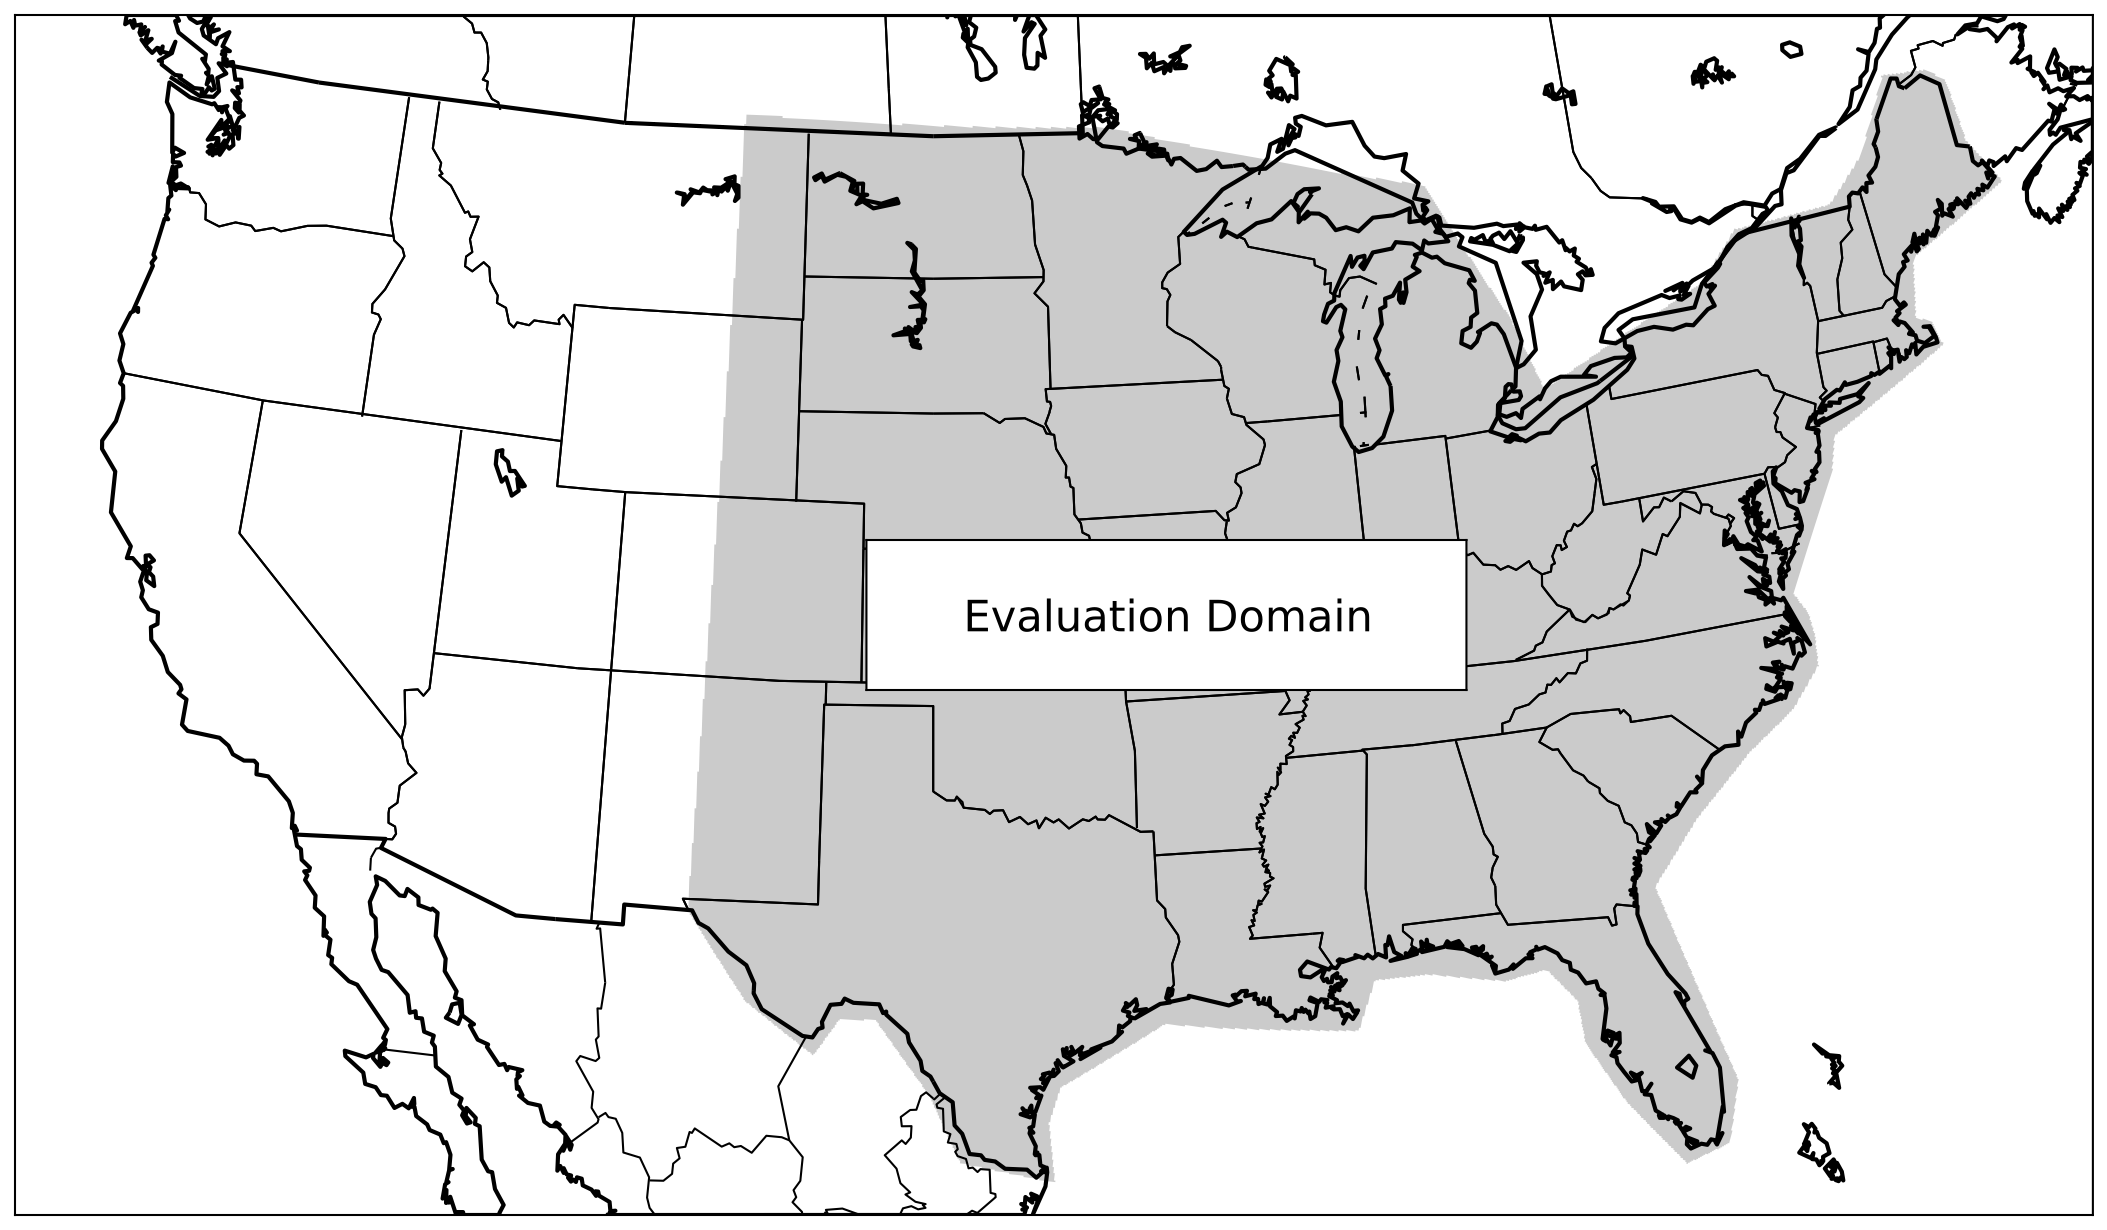
\includegraphics[width=\textwidth, height=\textheight, keepaspectratio]{%
    ./deterministic/figs/domain}\\
    \caption{The subset of the Stage IV grid used in the analysis.}
    \label{domain}
\end{figure}


\clearpage
\begin{figure}[cc]
    \centering
    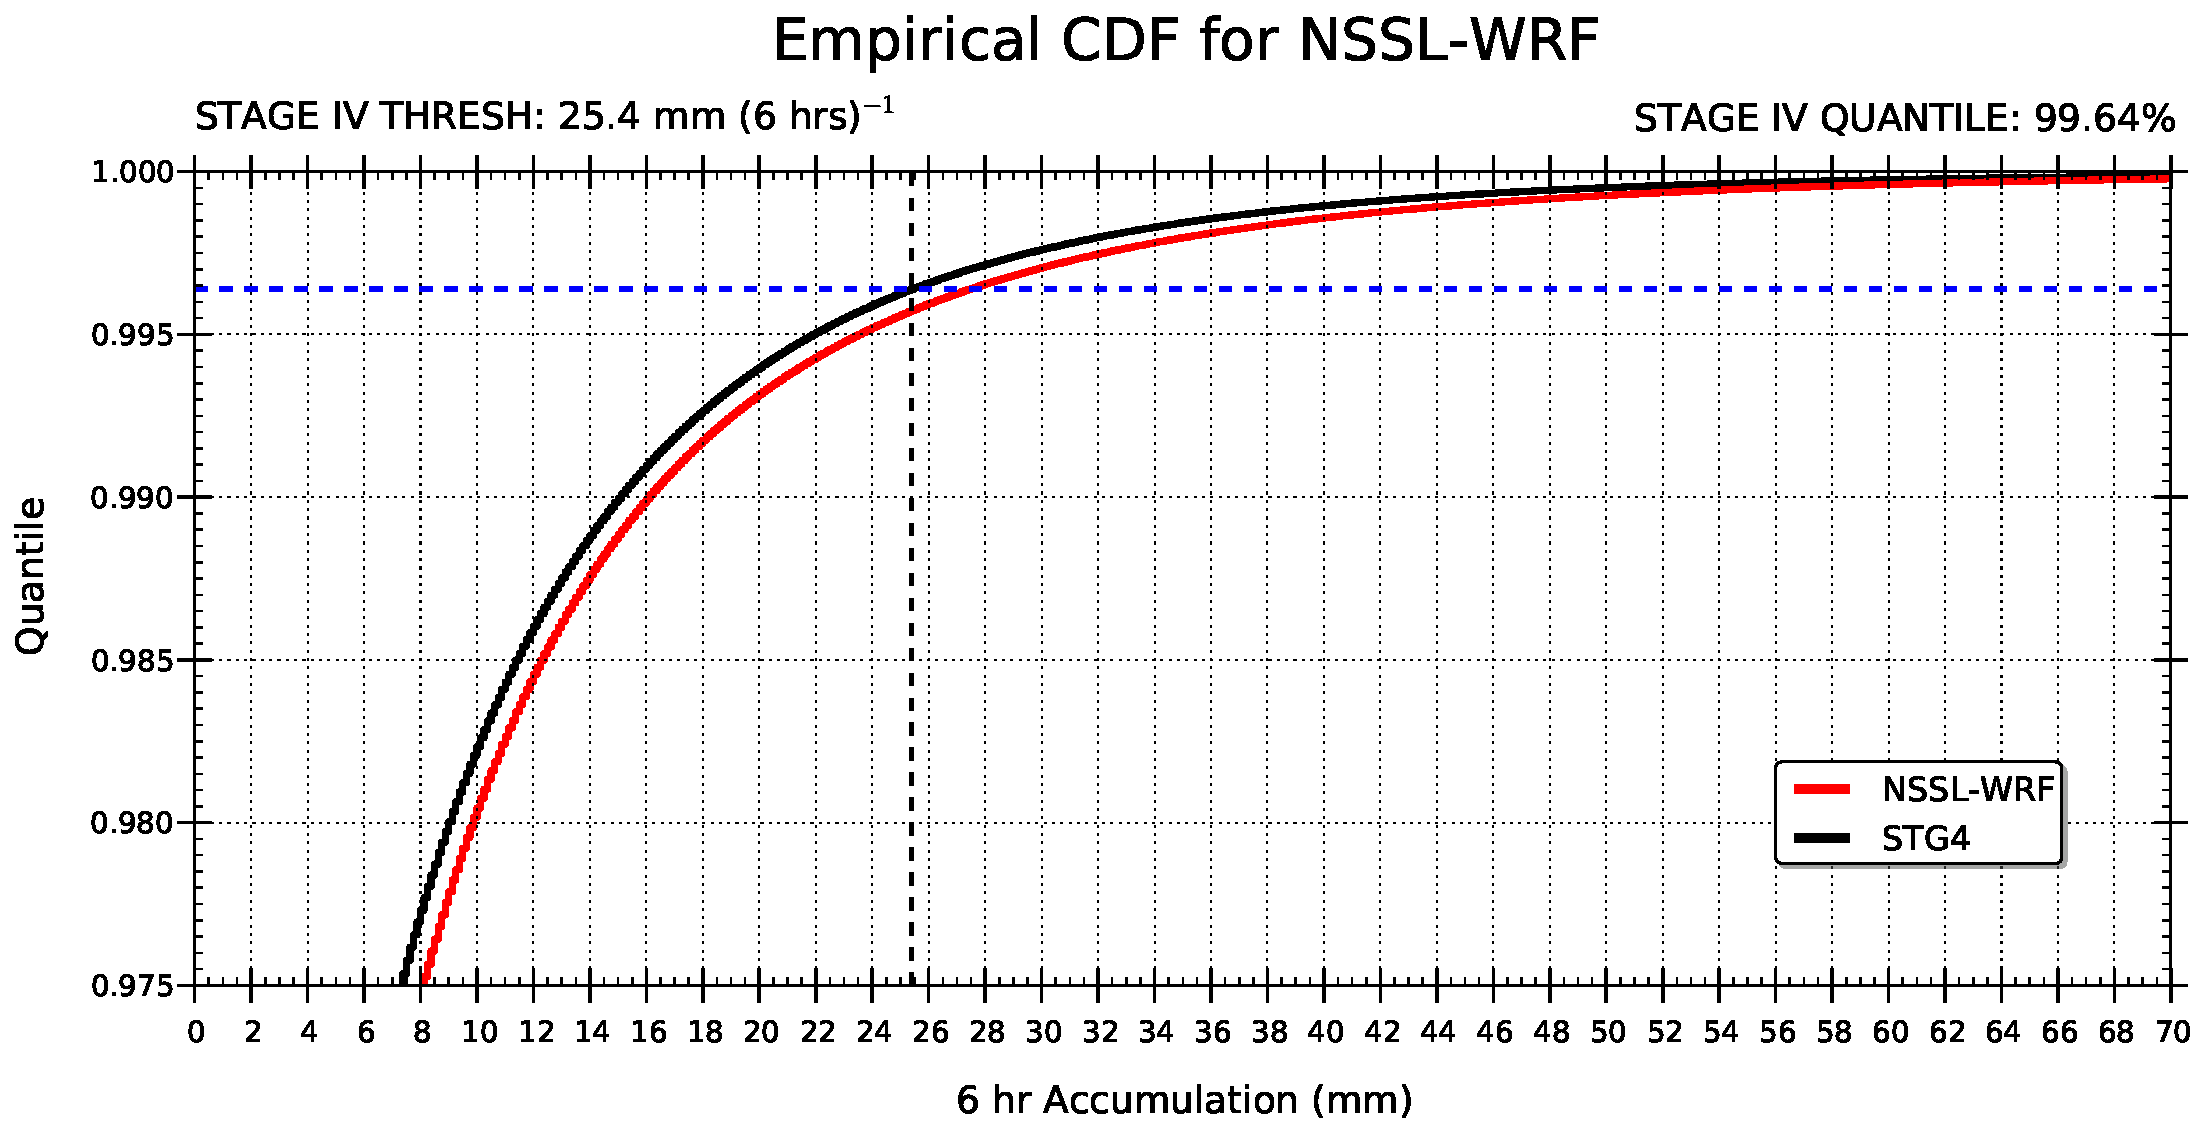
\includegraphics[width=\textwidth, height=\textheight, keepaspectratio]{%
    ./deterministic/figs/ecdf-nsslwrf-25mm}\\
    \caption{The empirical cumulative distribution function for both the Stage IV observations (black) and the NSSL-WRF forecasts (red), derived over the time period 01 April 2007 -- 31 March 2010.
    The vertical black dotted line is the \mbox{25.4 mm} threshold.
    The horizontal blue dotted line is the Stage IV quantile associated with the \mbox{25.4 mm} threshold.
    Where the blue dotted line intersects the NSSL-WRF empirical cumulative distribution function is the corresponding NSSL-WRF threshold at which the ratio of points above to points below is equal to the Stage IV ratio of points above to points below the \mbox{25.4 mm} threshold.
    This new threshold for the NSSL-WRF is \mbox{26.625 mm}.}
    \label{single_25quant}
\end{figure}


\clearpage
\begin{figure}[cc]
    \centering
    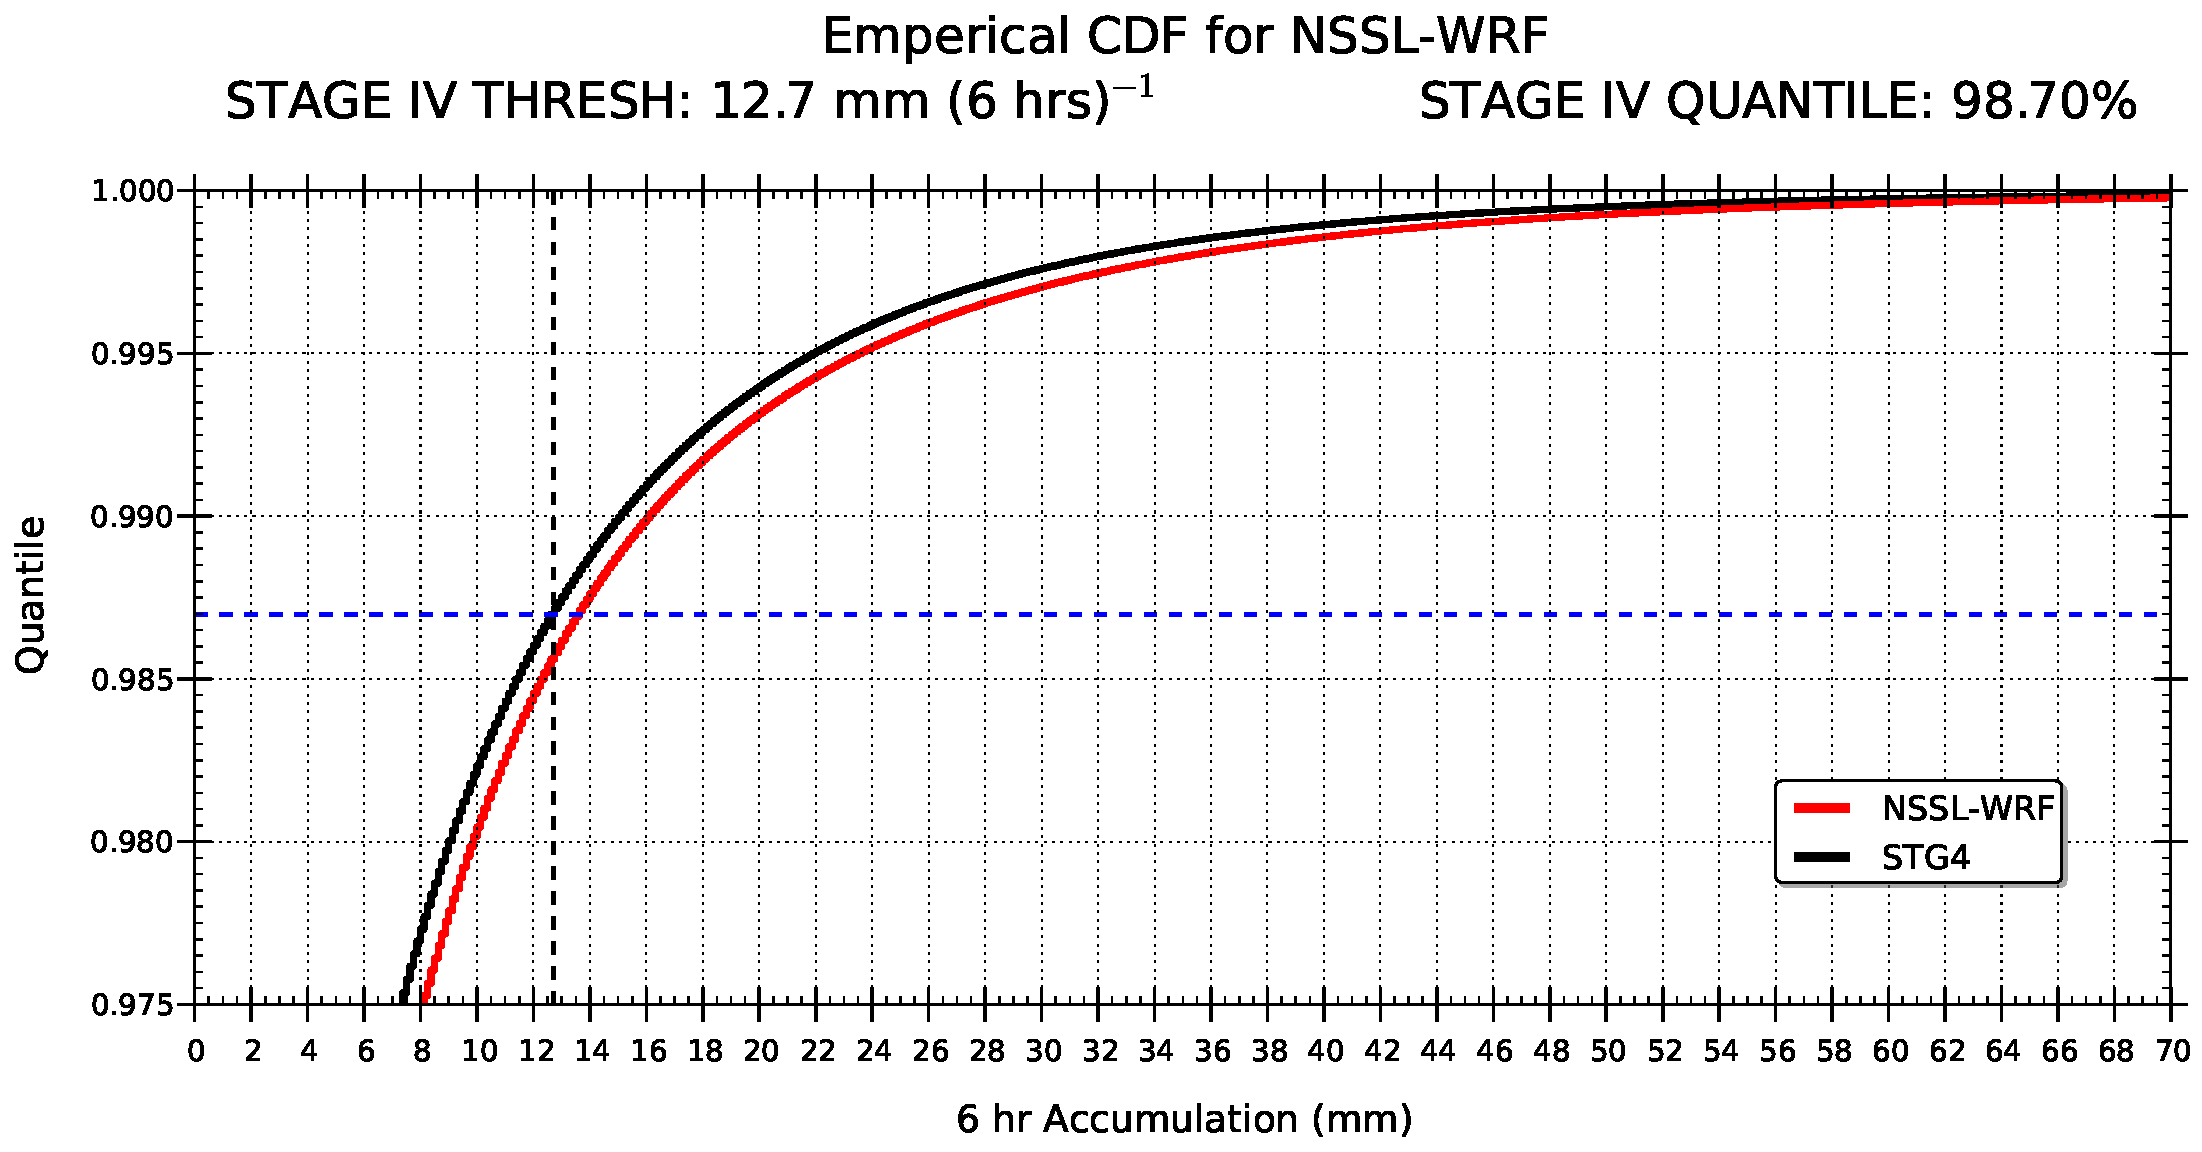
\includegraphics[width=\textwidth, height=\textheight, keepaspectratio]{%
    ./deterministic/figs/ecdf-nsslwrf-12mm}\\
    \caption{The same as in \mbox{Figure \ref{single_25quant}}, but using the \mbox{12.7 mm} threshold.
    The new threshold for the NSSL-WRF is \mbox{13.75 mm}.}
    \label{single_12quant}
\end{figure}


\clearpage
\begin{figure}[cc]
    \centering
    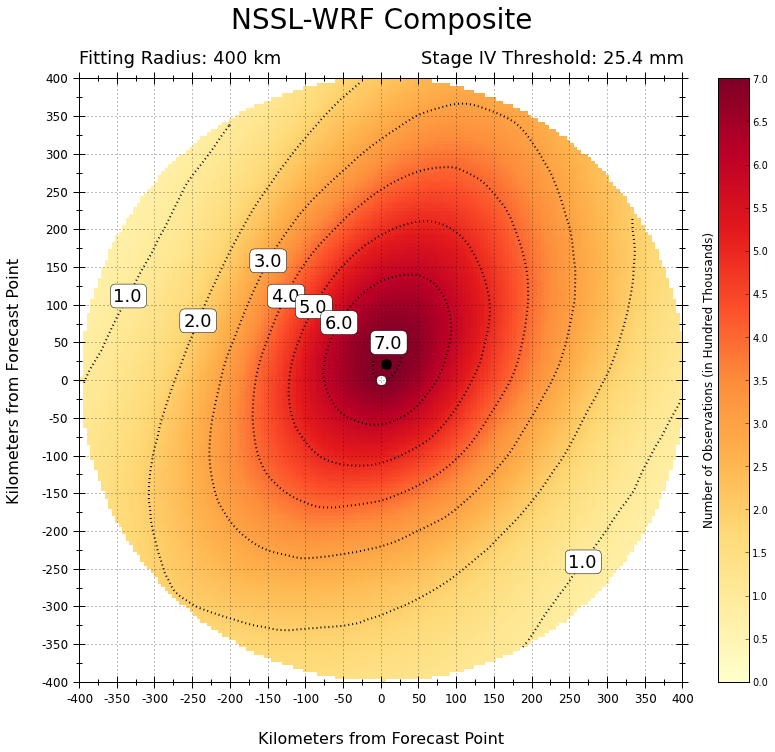
\includegraphics[width=\textwidth, height=\textheight, keepaspectratio]{%
    ./deterministic/figs/single_member_composite_400km_25mm}\\
    \caption{The two-dimensional frequency distribution of stage IV observations greater than or equal to \mbox{25.4 mm} relative to NSSL-WRF forecasts of similar events for the training dataset (1 Apr 2007 -- 31 Mar 2010).
    The representative NSSL-WRF forecast grid point is marked by a white dot in the middle of the domain and the stage IV observation frequency is color filled.
    To illustrate the displacement between forecasts and observations, the centroid of the observations is denoted by the black dot.
    Contour labels are given in hundred-thousands.}
    \label{single_25comp}
\end{figure}


\clearpage
\begin{figure}[cc]
    \centering
    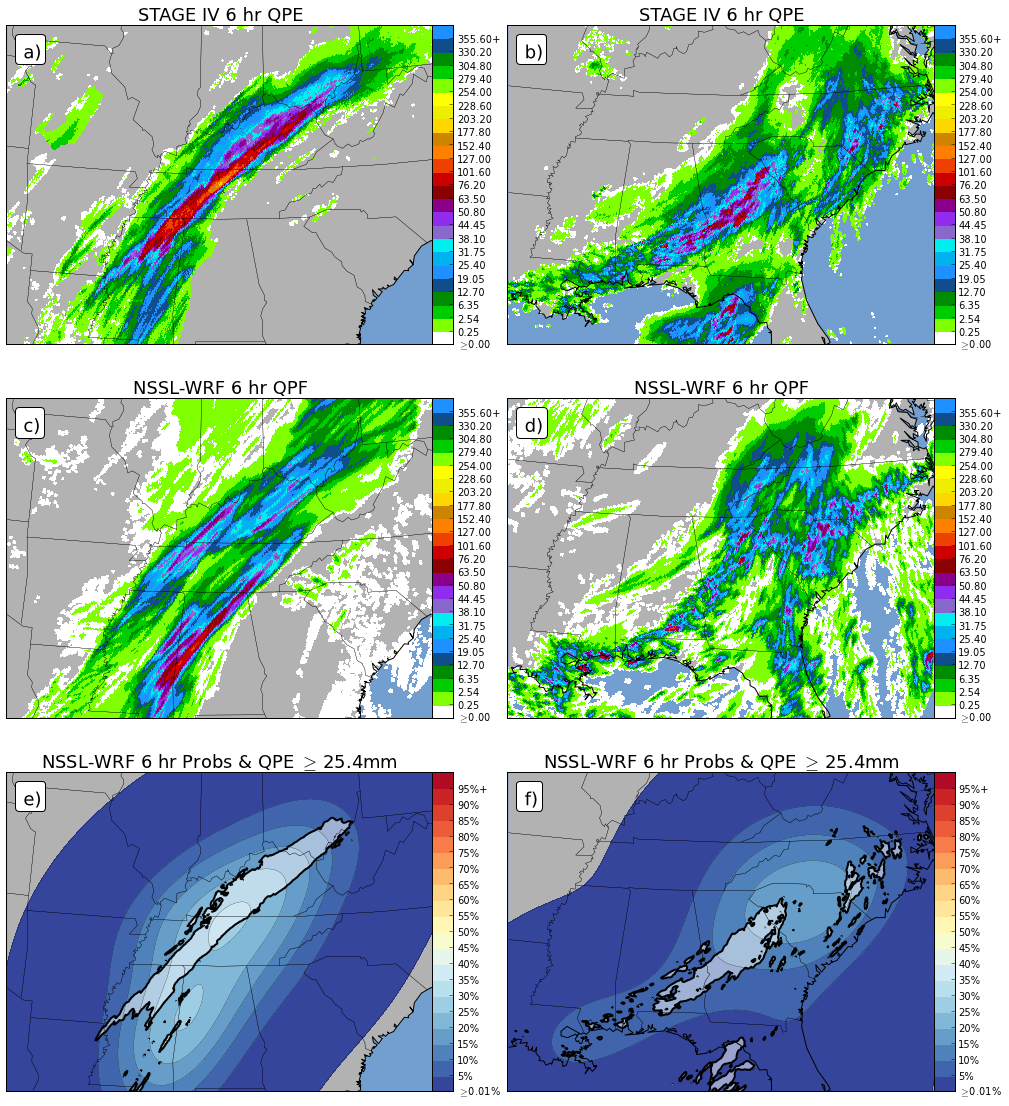
\includegraphics[width=\textwidth, height=\textheight, keepaspectratio]{%
    ./deterministic/figs/single_member_example1_400km_25mm}\\
    \caption{Example forecasts and observations from two separate days and differing forecast lengths.
    The column on the left depicts forecasts and observations for the 6-hrs ending 02 May 2010 at 18 UTC (12-18 hr forecast) whereas the column on the right depicts forecasts and observations for the 6-hrs ending 27 September 2010 at 00 UTC (18-24 hr forecast).
    The top panels denote the Stage IV 6-hr quantitative precipitation estimates (QPE), the middle panels denote the 6-hr NSSL-WRF 6-hr quantitative precipitation forecasts (QPF), and the bottom panels depict the Stage IV QPE greater than 25.4 mm contoured on top of the NSSL-WRF probability of exceeding 25.4 mm in 6-hrs. The minimum shaded probability is 0.0001 (0.01\%).}
    \label{single_1_400km_25mm}
\end{figure}


\clearpage
\begin{figure}[cc]
    \centering
    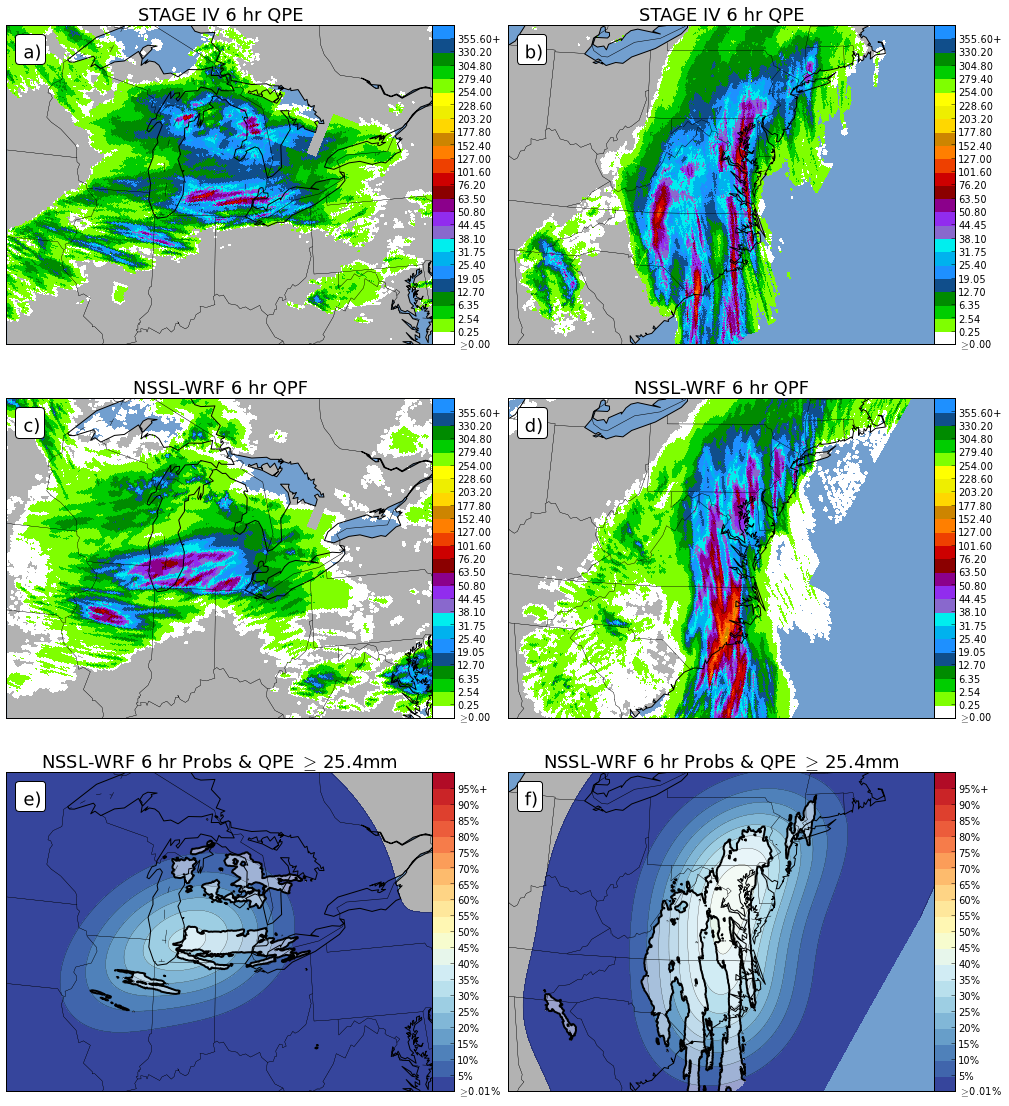
\includegraphics[width=\textwidth, height=\textheight, keepaspectratio]{%
    ./deterministic/figs/single_member_example2_400km_25mm}\\
    \caption{Same layout as in \mbox{Figure \ref{single_1_400km_25mm}} except the left column depicts the forecast and observations for the 6-hrs ending 06 June 2010 at 06 UTC (24-30 hr forecast) and the right column depicts the 6-hrs ending 30 September 2010 at 12 UTC (30-36 hr forecast).}
    \label{single_2_400km_25mm}
\end{figure}


\clearpage
\begin{figure}[cc]
    \centering
    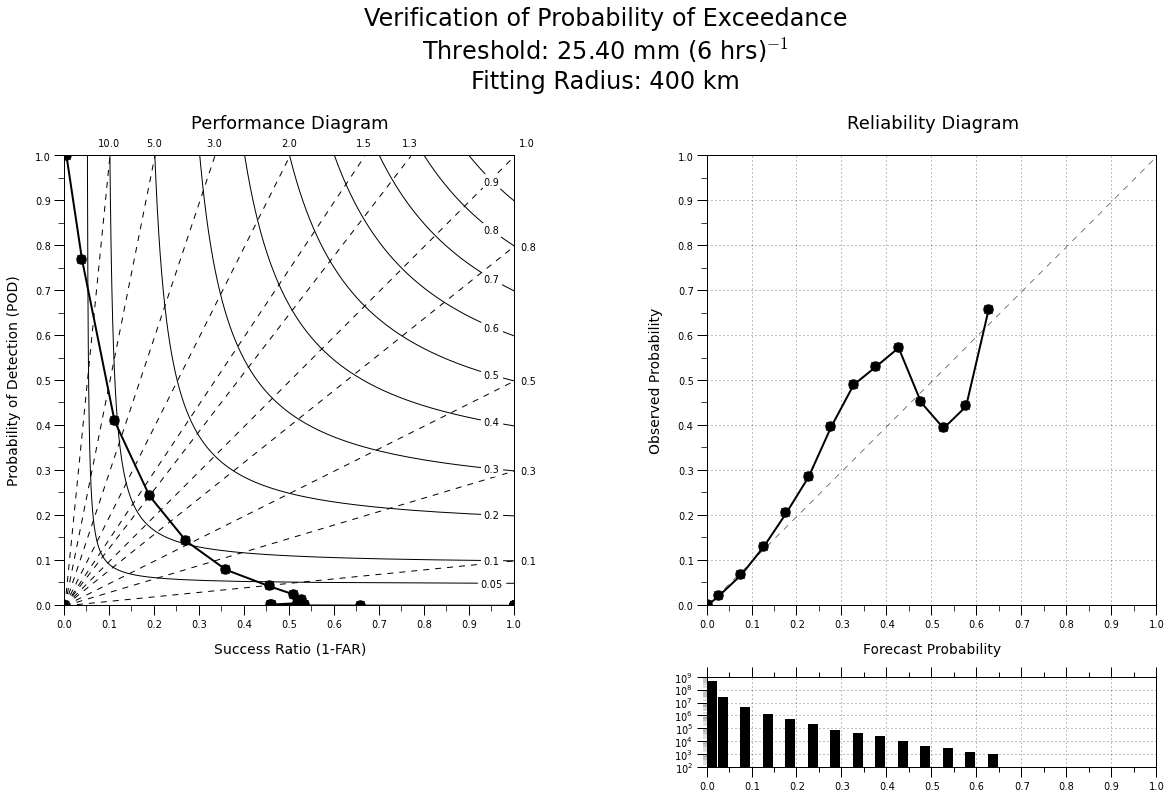
\includegraphics[width=\textwidth, height=\textheight, keepaspectratio]{%
    ./deterministic/figs/single_member_verif_400km_25mm}\\
    \caption{Performance Diagram (left) and reliability diagram with corresponding forecast counts (right), both computed over the 01 April 2010 to 31 March 2011 time period.
    The line of perfect reliability (diagonal; dashed) is also plotted on the reliability diagram.
    The forecast counts associated with the reliability diagram are plotted on a log-scale below the reliability diagram.}
    \label{single_verif_400km_25mm}
\end{figure}


\clearpage
\begin{figure}[cc]
    \centering
    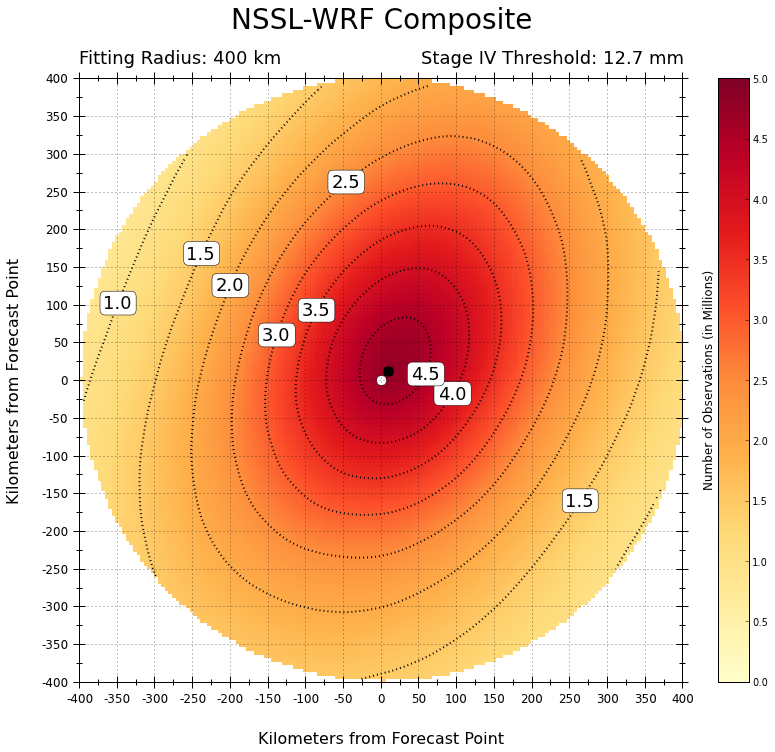
\includegraphics[width=\textwidth, height=\textheight, keepaspectratio]{%
    ./deterministic/figs/single_member_composite_400km_12mm}\\
    \caption{Same as in Figure \ref{single_25comp} except for the \mbox{12.7 mm} threshold and contour labels in millions.}

    \label{single_12comp}
\end{figure}


\clearpage
\begin{figure}[cc]
    \centering
    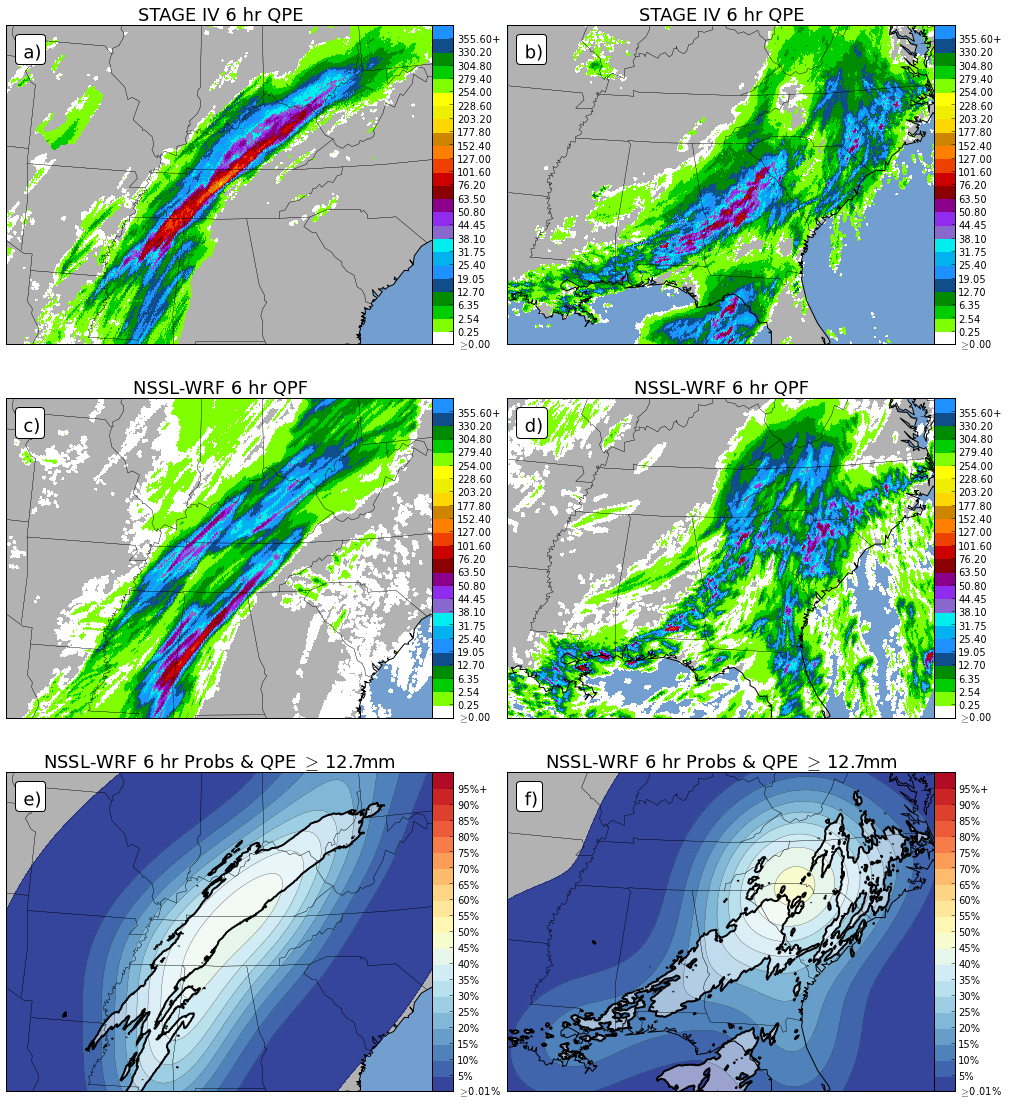
\includegraphics[width=\textwidth, height=\textheight, keepaspectratio]{%
    ./deterministic/figs/single_member_example1_400km_12mm}\\
    \caption{The same as in \mbox{Figure \ref{single_1_400km_25mm}} except using the \mbox{12.7 mm} threshold.}
    \label{single_1_400km_12mm}
\end{figure}


\clearpage
\begin{figure}[cc]
    \centering
    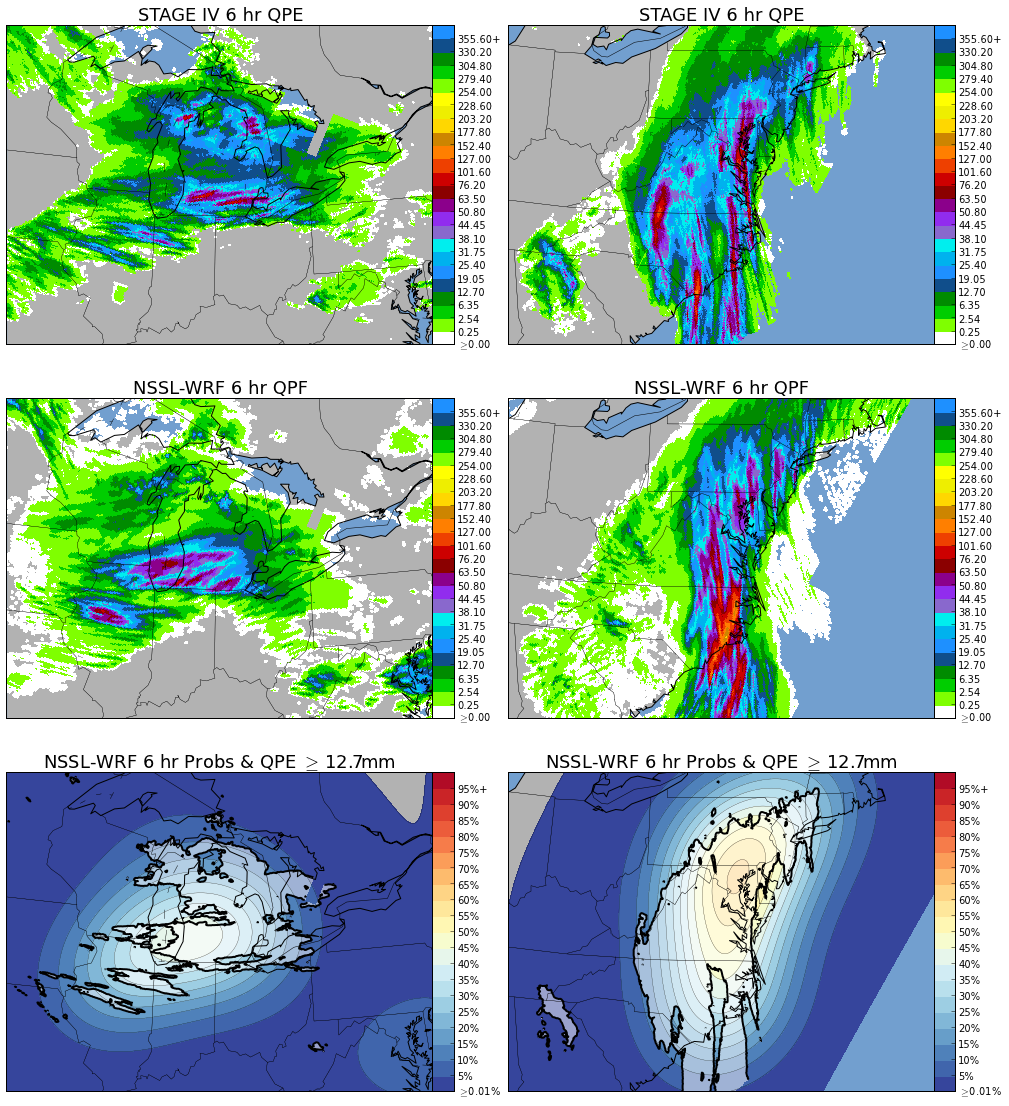
\includegraphics[width=\textwidth, height=\textheight, keepaspectratio]{%
    ./deterministic/figs/single_member_example2_400km_12mm}\\
    \caption{The same as in \mbox{Figure \ref{single_2_400km_25mm}} except using the \mbox{12.7 mm} threshold.}
    \label{single_2_400km_12mm}
\end{figure}


\clearpage
\begin{figure}[cc]
    \centering
    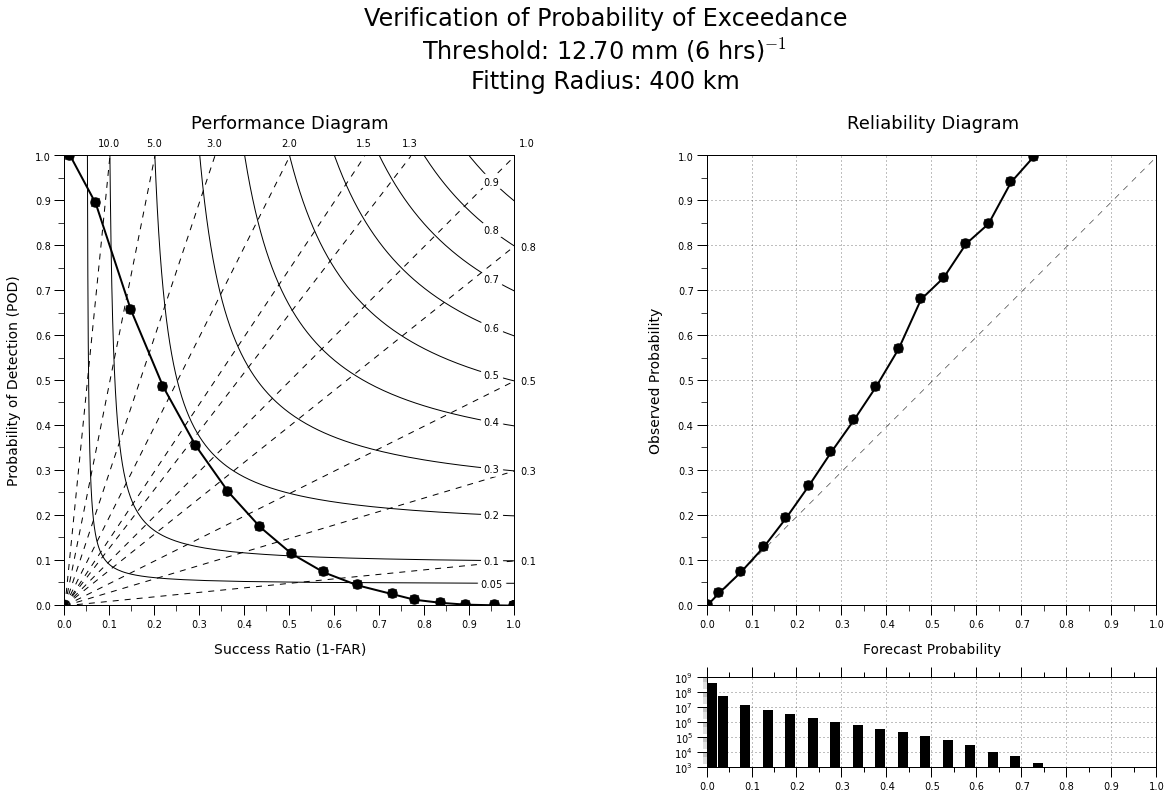
\includegraphics[width=\textwidth, height=\textheight, keepaspectratio]{%
    ./deterministic/figs/single_member_verif_400km_12mm}\\
    \caption{The same as in \mbox{Figure \ref{single_verif_400km_25mm}} except using the \mbox{12.7 mm} threshold.}
    \label{single_verif_400km_12mm}
\end{figure}






%!TEX root = ../dissertation.tex


\chapter{Ensemble}
\label{ensemble}



%!TEX root = ../dissertation.tex


\section{Ensemble Data}
\label{edata}




\subsection{Ensemble Forecasts}
\label{emodel}

As discussed at the beginning of \mbox{chapter \ref{deterministic}}, in order to develop a statistical post-processing method for calibration of numerical weather prediction forecasts, both forecasts and observations must be readily available.
Unfortunately, as mentioned in the Introduction, ``\dots there is a limited database of forecasts for RCEs, making robust statistical techniques difficult\dots''
As limited as databases of deterministic CAM forecasts are, the availability of \emph{ensembles} of CAM forecasts is even worse.


Similar to CAM forecasts, most storm-scale ensemble forecast systems\footnote{The phrase storm-scale ensemble forecast is typically used in reference to ensembles composed of numerical forecasts produced without using cumulus parameterization.} (SSEF) have been erected on a temporary basis, produced in support of various field programs and experiments.
The makeup of these SSEFs are often modified from one program to the next to adapt to the changing needs of the various experiments.
Long running, consistent configured SSEFs were not available for this work.
It is worth noting that as this work neared completion, the Air Force Weather Agency began running an operational SSEF.


One of the largest collections of SSEF forecasts has been produced by the University of Oklahoma's Center for the Analysis and Prediction of Storms (CAPS).
Since 2007, CAPS has been producing CAM forecasts in support of the Hazardous Weather Testbed's (HWT) annual Spring Forecast Experiment (SFE).
From 2007 through 2010, the ensemble configuration changed from year-to-year based on the results of previous years and updated to the WRF modeling system.
In 2010, CAPS produced a 26 member SSEF.
This SSEF was multi-model in nature, initialized at 00 UTC, used 4 km grid spacing, and integrated out to 30 hours.
Of the 26 members, 19 were WRF-ARW\footnote{Weather Research and Forecasting -- Advanced Research WRF} \citep{WRFV3}, 5 were WRF-NMM\footnote{Weather Research and Forecasting -- nonhydrostatic Mesoscale Model} \citep{NAMnWRF-NMM}, and 2 were ARPS\footnote{Advanced Regional Prediction System} \citep{ARPS}.
In 2011, CAPS expanded the SSEF from 26 members to 50, of which 41 were WRF-ARW, 5 were WRF-NMM, and 4 were ARPS.
These forecasts were also initialized at 00 UTC, used a grid spacing of 4 km, but were integrated forward to 36 hours instead of 30.


For this thesis, fifteen members were chosen from the 2010 and 2011 ensembles because these members were configured almost identically between the two years.
These 15 members were composed of 10 WRF-ARW forecasts, 4 WRF-NMM forecasts, and 1 ARPS forecast.
The background initial conditions for these 15 members were downscaled from the 00 UTC 12 km NAM, with additional information coming from a three dimensional variational and cloud analysis from ARPS.
Except for the control members (one each from the WRF-ARW, WRF-NMM, and ARPS), these initial conditions were then perturbed using mesoscale atmospheric perturbations from NOAA's Environmental Modeling Center's operational Short-Range Ensemble Forecast (SREF) system.
Lateral boundary conditions for the three control members came from the 00 UTC NAM forecasts, whereas the remaining 12 members used the SREF forecast corresponding to the perturbations used in the initial conditions.
A listing of the configurations for each member of the SSEF can be found in \mbox{Table \ref{ensemble_members}}.


The only controlled change between 2010 and 2011 for the aforementioned set of 15 forecasts came from a change in the version of WRF. In 2010, \mbox{WRF Version 3.1.1} was used whereas \mbox{WRF Version 3.2.1} was used in 2011.
Changes in the NAM and SREF, which were used for initial and lateral boundary conditions, were controlled by the NOAA National Weather Service and could not be avoided.


In 2010 the HWT SFE ran from 17 May through 18 June, and in 2011, the HWT SFE ran from 09  May through 10 June.
CAPS provided SSEF forecasts each weekday during the experiment, with an additional two retrospective forecasts in 2011: one for the 27 April 2011 tornado outbreak in the southeast United States and another for the 22 May 2011 Joplin, Missouri EF-5 tornado.
\mbox{Table \ref{sfedtes}} lists the dates for which CAPS forecasts are available.


In an effort to be consistent with the evaluation carried out on the NSSL-WRF, the decision was made to use six-hour accumulation periods for the SSEF forecasts\footnote{Unless otherwise noted, from this point forward the phrase ``SSEF'', ``SSEF forecasts'', or variants thereof refer to the 15 numerical forecasts that are presented in \mbox{Table \ref{ensemble_members}}.} and the Stage IV analyses.
As was the case with the NSSL-WRF, the SSEF forecasts were drawn from subsets of the \mbox{12-36 hr} forecast period ending at 18, 00, 06, and 12 UTC, but only for \mbox{6 hr} time periods for which every member was available.
Because the 2010 SSEF was only integrated out to \mbox{30 hr}, the potential dataset was immediately reduced to 156 six-hour time periods (52 days times 3 periods a day).




\subsection{Observations}
\label{eobservations}

As was the case for the evaluating the deterministic model calibration, NCEP's Stage IV national quantitative precipitation estimate analysis was chosen as the verification dataset.
Please see \mbox{section \ref{observations}} for a description of the Stage IV dataset.




\subsection{Processing}
\label{eprocessing}

As stated in \mbox{section \ref{emodel}}, there were a maximum of 156 six-hour time periods for which SSEF data was expected.
This potential dataset was further thinned by removing all time periods in which either one or more SSEF members were missing or the Stage IV analysis was unavailable.
An additional 37 six-hour time periods were removed as a result, leaving 119 six-hour time periods, over 2010 and 2011, for which both the entire SSEF and the Stage IV analyses are available.


Next, as was necessary with the deterministic forecasts, the ensemble forecasts were interpolated to the Stage IV grid.
All diagnostics and analyses were conducted on this grid.
Furthermore, the same mask shown in \mbox{Figure \ref{domain}} was used to limit the analyses to areas east of the Rocky Mountains and near land.


Unfortunately, 119 time periods is a very small sample from which to evaluate a method for statical calibration of forecasts of rare events.
This is especially true when the training and forecast data must both come from the 119 time periods.
For comparison, the NSSL-WRF training dataset had 4120 training time periods and 1425 forecast time periods.
In an attempt to maximize the utility of the 119 time periods, twenty ``simulations'' were created by resampling the 119 time periods.
This was accomplished by randomly drawing, without replacement, 59 training periods from the valid 119 time periods with the remaining 60 periods used as forecast periods.
From these 59 training periods, two-dimensional histograms were created for each of the 15 ensemble members.
These histograms were then used to calculate the five fitting parameters --- $\sigma_x$, $\sigma_y$, $\theta$, $h$, and $k$ --- for each member's unique two-dimensional anisotropic Gaussian function.
Forecasts for each member were then made for each time period of the 60 forecast time periods, with each member using its own fitted anisotropic Gaussian function.
Thus, for each simulation all 15 ensemble members used the same 59 time periods for training and the remaining 60 time periods for forecasting.
This results in 18 000 forecasts (20 simulations x 60 forecast periods x 15 members).







%!TEX root = ../dissertation.tex


\section{Ensemble Results}
\label{eresults}




\subsection{25.4 mm Threshold}
\label{eresults_25.4mm}

As previously mentioned, the first step of the proposed calibration process is to create two-dimensional composites of where observations occurred relative to forecast grid points.
In the case of the small number of SSEF forecasts, this amounts to creating a composite for each member for each simulation.
\mbox{Figure \ref{ssef-25mm-400km-composite}} shows the the two-dimensional composites for each member at the \mbox{25.4 mm} in \mbox{6 hr} threshold for one of the twenty simulations.
In this simulation, it is readily apparent that the WRF-NMM ensemble members are generaly the wettest, with the WRF-ARW members drier.
(The ARPS member is in between.)
The overall axis of observations relative to forecasts indicates a general southeast-to-northeast orientation in most members, although this is more readily apparent in some members than others.


Although the orientation of the axis of maximum observations tends to generally be similar between members, the centroid of the distribution exhibits more variability.
About half of the members have the centroid of observations too far east and half having the centroid be too far west.
(This corresponds to the $h$ parameter of the Gaussian fitting parameters.)
The members having the observations centroid too far east tended to be farther away from the forecast than those members having the observations centroid too far west.
In this simulation, the WRF-NMM has a westward bias with its forecasts, as the centroid of observations is east of the forecast grid point in every WRF-NMM member.
A similar observation cannot be made for the WRF-ARW members.
It is unclear from this single simulation if the westward forecast bias in the WRF-NMM members is systematic of the WRF-NMM core, or merely a function of only having 4 WRF-NMM members.


When examining the north/south variations of the observations centroid relative to the model forecast, similar variations are observed.
(The north/south displacement of the observations centroid corresponds to the $k$ parameter of the Gaussian fitting parameters.)
Slightly more than half the members have the centroid of observations too far north, indicating a southward bias of the forecast, with slightly less than half having the centroid of observations too far south.
Three of the four WRF-NMM members had the forecast too far north, with the WRF-NMM control member having the greatest displacement.
No obvious preference in displacement direction is readily apparent from the WRF-ARW members.
However, it does appear that generally speaking, the magnitude of the displacement of the WRF-ARW members appears to be less than that of the WRF-NMM members.


The lower right panel of \mbox{Figure \ref{ssef-25mm-400km-composite}} depicts the standard deviation between the two-dimensional composites of each member for the given simulation.
In this panel, the darker colors indicate a greater standard deviation at that particular grid point than grid points with a lighter color.
It is readily apparent that the greatest variability between the members exists to the east of the forecast grid point.
This is due to the wetter WRF-NMM members having a westward forecast bias, resulting in a wider range of observation counts to the east of the forecast.


Unfortunately, \mbox{Figure \ref{ssef-25mm-400km-composite}} is only one simulation out of the twenty simulations produced.
In an attempt to gain insights into the variation of the two-dimensional composites for each member between all twenty simulations, the standard deviation of each member's composites is shown in \mbox{Figure \ref{ssef-25mm-400km-std}}.
A cursory examination of the standard deviation of the two-dimensional composites does not yield any immediate insights.
Some members exhibit a maximum in variability along a southwest to northeast orientation.
Other members exhibit a more uniform increase in the maximum variability.
In both cases, the maximum variability tended to be located near the forecast grid point, with generally decreasing variability as distance from the forecast grid point increases.


Breaking down the fitting parameters by simulation gives an even better idea of the variability in each member's twenty two-dimensional composites.
A set of five figures (\mbox{Figures \ref{sigmax-25mm-400km-dist}--\ref{k-25mm-400km-dist}}) were created to examine the variability of each of the five Gaussian fitting parameters --- one figure per fitting parameter.
The figures contain box-and-whisker plots for each member's distribution of that figure's fitting parameter.
The box-and-whisker plots offer insight into the variability in the various fitting functions used by each member.
In each of the figures, the red horizontal line marks the median value of the distributions, and the blue box represents the 25th and 75th percentiles.
The whiskers denote the range of the distribution, up to $\pm$ 1.5 times the interquartile range.
Gold stars are used to denote any outliers, defined to be any value of the distribution that is outside the range of $\pm$ 1.5 times the interquartile range.


\mbox{Figure \ref{sigmax-25mm-400km-dist}} displays the box-and-whisker plots for the $\sigma_x$ fitting parameter.
This parameter is the length of the long axis of the fitted anisotropic Gaussian function.
Nine out of the fifteen ensemble members do not have outliers.
Of the remaining six ensemble members with outliers, two of them only have one outlier, two of them have two outliers, and one each has four and five outliers.
Ensemble members that have outliers had a range of over 20 kilometers for $\sigma_x$, whereas those members without outliers generally had ranges of less than 20 kilometers.
This means that 40\% of the ensemble members had variability in their $\sigma_x$ parameter that was greater than 10\% of the median length of the $\sigma_x$ fitting parameter.


\mbox{Figure \ref{sigmay-25mm-400km-dist}} shows the box-and-whisker plots for the $\sigma_y$ fitting parameter.
This parameter is the length of the short axis of the fitted anisotropic Gaussian function.
Unlike with the $\sigma_x$ fitting parameter, the ensemble member distributions of the $\sigma_y$ fitting parameter exhibit fewer outliers with only four members having them.
This can be attributed to their being more variability in the 25th to 75th percentile, as noted by the increased size of the boxes for many members.
Furthermore, whereas when the maximum range of the $\sigma_x$ fitting parameter distribution greater than 20 kilometers indicated the presence of an outlier, several members have distributions of $\sigma_y$ with a maximum range greater than 20 kilometers without having an outlier.
In fact, six out of the ten WRF-ARW members have a range of $\sigma_y$ greater than 20 kilometers and only two of them have outliers.


The distributions of the counter-clockwise rotation angle of the abscissa, fitting parameter $\theta$, is shown in \mbox{Figure \ref{theta-25mm-400km-dist}}.
For this fitting parameter, eleven out of fifteen members exhibit outliers.
This is not really surprising when one considers the overlap in the distributions of fitting parameters $\sigma_x$ and $\sigma_y$.
As alluded to in \mbox{Section \ref{std}}, when $\sigma_x$ approaches $\sigma_y$, the Gaussian function approaches being isotropy.
As a Gaussian function approaches isotropy the variability of the rotation angle, $\theta$ increases as a result of the more circular nature to the function.
It is much more difficult to accurately measure the orientation of the rotation angle of an ellipse that is nearly circular than that of one with a high level of eccentricity.


The variability in the fitting parameters was not limited to just the shape of the anisotropic Gaussian.
The location of the fitting Gaussian also ranged widely.
Each member's distributions of the $h$ fitting parameter (displacement in the east or west direction) is shown in \mbox{Figure \ref{h-25mm-400km-dist}}.
Generally speaking, some of the values for $h$ deviated from the forecast grid point by over 40 kilometers.
The ARPS and WRF-NMM members consistently demonstrated a bias toward the observations centroid being east.
This corresponds to the forecasts, on average, being too far west compared to where observations occurred.
Most of the WRF-ARW members exhibited the opposite behavior, namely having the observations being too far east (indicating an eastward bias with the forecast).
Not every WRF-ARW member exhibited this bias, however.
The values comprising the interquartile range for two of the WRF-ARW members consisted of positive values for $h$, indicating a westward forecast bias.
However, unlike with the ARPS and WRF-NMM members, where the entire distribution consisted of positive values for $h$, every member of the WRF-ARW had at least a portion of the ``whiskers'' part of the box-and whiskers plot with negative values, indicating an eastward forecast bias, as compared to observations.



















% table definitions
%%%%%%%%%%%%%%%%%%%
\newenvironment{telement}[2]{\begin{minipage}[c]{#1} \centering #2} {\end{minipage}}
\newcommand{\coremem}{\color{red}}
\newcommand{\member}[1]{\begin{telement}{0.75in}{#1}\end{telement}}
\newcommand{\ic}[1]{\begin{telement}{1in}{#1}\end{telement}}
\newcommand{\bc}[1]{\begin{telement}{0.75in}{#1}\end{telement}}
\newcommand{\radar}[1]{\begin{telement}{0.75in}{#1}\end{telement}}
\newcommand{\microphysics}[1]{\begin{telement}{0.75in}{#1}\end{telement}}
\newcommand{\lsm}[1]{\begin{telement}{0.75in}{#1}\end{telement}}
\newcommand{\pbl}[1]{\begin{telement}{0.75in}{#1}\end{telement}}

\newpage

\begin{center}
    \renewcommand{\arraystretch}{3}
    \centering
    \singlespace
    \small
    \setlength\tabcolsep{2pt}
    \rowcolors{2}{gray!20}{white}
    \begin{longtable}{|c|c|c|c|c|c|c|}
        \caption[Configurations for the 2010 and 2011 CAPS Ensemble Members]
        {Configurations for the 2010 and 2011 CAPS Ensemble Members.}
        \label{ensemble_members} \\

        % Header for the first page
        \hline
        \rowcolor{gray!60}
        \member{\textbf{Member}} &
        \ic{\textbf{I. C.}} &
        \bc{\textbf{B. C.}} &
        \radar{\textbf{Radar}} &
        \microphysics{\textbf{Micro-\\physics}} &
        \lsm{\textbf{LSM}} &
        \pbl{\textbf{PBL}} \\
        \hline
        \endfirsthead

        % Header for remaining pages
        \hline
        \multicolumn{7}{|c|}{{\tablename} \thetable{} -- Continued} \\
        \hline
        \rowcolor{gray!60}
        \member{\textbf{Member}} &
        \ic{\textbf{I. C.}} &
        \bc{\textbf{B. C.}} &
        \radar{\textbf{Radar}} &
        \microphysics{\textbf{Micro-\\physics}} &
        \lsm{\textbf{LSM}} &
        \pbl{\textbf{PBL}} \\
        \hline
        \endhead

        %This is the footer for all pages except the last page of the table...
        \multicolumn{7}{|c|}{{Continued on Next Page \ldots}} \\
        \hline
        \endfoot

        %This is the footer for the last page of the table...
        \hline
        \multicolumn{7}{|l|}{Note 1: For all members, cumulus parameterization is turned off} \\
        \hline
        \multicolumn{7}{|l|}{\multirow{1}{\textwidth}{Note 2: For all ARW members, the long-wave radiation parameterization is RRTM and the short-wave radiation parameterization is Goddard}} \\
        \hline
        \multicolumn{7}{|l|}{\multirow{1}{\textwidth}{Note 3: For nmm\_cn, nmm\_m2, \& nmm\_m3 the long-wave radiation parameterization is GFDL and the short-wave radiation parameterization is GFDL}} \\
        \hline
        \multicolumn{7}{|l|}{\multirow{1}{\textwidth}{Note 4: For nmm\_m4 \& nmm\_m5 the long-wave radiation parameterization is RRTM and the short-wave radiation parameterization is Dudhia}}\\
        \hline
        \multicolumn{7}{|l|}{Note 5: The arps member uses Chou/Suarex for radiation} \\
        \hline
        \multicolumn{7}{|l|}{Note 6: Ferrier+ refers to a subset of changes in the updated version now in NEMS/NMMB} \\
        \hline
        \multicolumn{7}{|l|}{\multirow{1}{\textwidth}{Note 7: The ARPS PBL scheme \citep{Xue1996, Sun1986} uses a non-local vertical mixing length within the convective boundary layer}} \\
        \hline
        \endlastfoot

        % Member 1 of 24
        \hline
        \coremem\member{arw\_cn} &
        \coremem\ic{00Z ARPS 3DVAR \& Cloud Analysis} &
        \coremem\bc{00Z NAM Forecast} &
        \coremem\radar{Yes} &
        \coremem\microphysics{Thompson} &
        \coremem\lsm{Noah} &
        \coremem\pbl{MYJ} \\

        % Member 2 of 24
        \hline
        \coremem\member{arw\_m4} &
        \coremem\ic{arw\_cn + em\_p1\_pert} &
        \coremem\bc{21Z SREF em\_p1} &
        \coremem\radar{Yes} &
        \coremem\microphysics{Morrison} &
        \coremem\lsm{RUC} &
        \coremem\pbl{YSU} \\

        % Member 3 of 24
        \hline
        \coremem\member{arw\_m5} &
        \coremem\ic{arw\_cn + em\_p2\_pert} &
        \coremem\bc{21Z SREF em\_p2} &
        \coremem\radar{Yes} &
        \coremem\microphysics{Thompson} &
        \coremem\lsm{Noah} &
        \coremem\pbl{QNSE} \\

        % Member 4 of 24
        \hline
        \coremem\member{arw\_m6} &
        \coremem\ic{arw\_cn - nmm\_p1\_pert} &
        \coremem\bc{21 SREF nmm\_p1} &
        \coremem\radar{Yes} &
        \coremem\microphysics{WSM6} &
        \coremem\lsm{RUC} &
        \coremem\pbl{QNSE} \\

        % Member 5 of 24
        \hline
        \coremem\member{arw\_m7} &
        \coremem\ic{arw\_cn + nmm\_p2\_pert} &
        \coremem\bc{21Z SREF nm\_p2} &
        \coremem\radar{Yes} &
        \coremem\microphysics{WDM6} &
        \coremem\lsm{Noah} &
        \coremem\pbl{MYNN} \\

        % Member 6 of 24
        \hline
        \coremem\member{arw\_m8} &
        \coremem\ic{arw\_cn + rsm\_n1\_pert} &
        \coremem\bc{21Z SREF rsm\_n1} &
        \coremem\radar{Yes} &
        \coremem\microphysics{Ferrier} &
        \coremem\lsm{RUC} &
        \coremem\pbl{YSU} \\

        % Member 7 of 24
        \hline
        \coremem\member{arw\_m9} &
        \coremem\ic{arw\_cn - etaKF\_n1\_pert} &
        \coremem\bc{21Z SREF etaKF\_n1} &
        \coremem\radar{Yes} &
        \coremem\microphysics{Ferrier} &
        \coremem\lsm{Noah} &
        \coremem\pbl{YSU} \\

        % Member 8 or 24
        \hline
        \coremem\member{arw\_m10} &
        \coremem\ic{arw\_cn + etaKF\_p1\_pert} &
        \coremem\bc{21Z SREF etaKF\_p1} &
        \coremem\radar{Yes} &
        \coremem\microphysics{WDM6} &
        \coremem\lsm{Noah} &
        \coremem\pbl{QNSE} \\

        % Member 9 of 24
        \hline
        \coremem\member{arw\_m11} &
        \coremem\ic{arw\_cn - etaBMJ\_p1\_pert} &
        \coremem\bc{21Z SREF etaBMJ\_p1 } &
        \coremem\radar{Yes} &
        \coremem\microphysics{WSM6} &
        \coremem\lsm{RUC} &
        \coremem\pbl{MYNN} \\

        % Member 10 of 24
        \hline
        \coremem\member{arw\_m12} &
        \coremem\ic{arw\_cn + etaBMJ\_p1\_pert} &
        \coremem\bc{21Z SREF etaBMJ\_p1} &
        \coremem\radar{Yes} &
        \coremem\microphysics{Thompson} &
        \coremem\lsm{RUC} &
        \coremem\pbl{MYNN} \\

        % Member 19 of 24
        \hline
        \coremem\member{nmm\_cn} &
        \coremem\ic{00Z ARPS 3DVAR \& Cloud Analysis} &
        \coremem\bc{00Z NAM Forecast} &
        \coremem\radar{Yes} &
        \coremem\microphysics{Ferrier} &
        \coremem\lsm{Noah} &
        \coremem\pbl{MYJ} \\

        % Member 21 of 24
        \hline
        \coremem\member{nmm\_m3} &
        \coremem\ic{nmm\_cn + nmm\_n1\_pert} &
        \coremem\bc{21Z SREF nmm\_n1} &
        \coremem\radar{Yes} &
        \coremem\microphysics{Thompson} &
        \coremem\lsm{Noah} &
        \coremem\pbl{MYJ} \\

        % Member 22 of 24
        \hline
        \coremem\member{nmm\_m4} &
        \coremem\ic{arw\_cn + nmm\_n2\_pert} &
        \coremem\bc{21Z SREF nmm\_n2} &
        \coremem\radar{Yes} &
        \coremem\microphysics{WSM6} &
        \coremem\lsm{RUC} &
        \coremem\pbl{MYJ} \\

        % Member 23 of 24
        \hline
        \coremem\member{nmm\_m5} &
        \coremem\ic{arw\_cn + em\_n1\_pert} &
        \coremem\bc{21Z SREF em\_n1} &
        \coremem\radar{Yes} &
        \coremem\microphysics{Ferrier} &
        \coremem\lsm{RUC} &
        \coremem\pbl{MYJ} \\

        % Member 24 or 24
        \hline
        \coremem\member{arps\_cn} &
        \coremem\ic{00Z ARPS 3DVAR \& Cloud Analysis} &
        \coremem\bc{00Z NAM Forecast} &
        \coremem\radar{Yes} &
        \coremem\microphysics{Lin} &
        \coremem\lsm{Force Restore} &
        \coremem\pbl{1.5-order TKE-based} \\
        \hline

    \end{longtable}
\end{center}




\begin{table}[cc]
    \centering
    \setlength{\tabcolsep}{0.5in}
    \renewcommand{\arraystretch}{1.25}
    \caption[2010 and 2011 dates where CAPS forecasts are available.]
    {2010 and 2011 dates where CAPS forecasts are available.}
    \label{sfedtes} \vspace{0.25in}
    \begin{tabular}{||c c||}
        \hline \hline
        \vspace{\baselineskip} & \vspace{\baselineskip} \\
        \multicolumn{2}{||c||}{\Large 2010 Dates} \\
        \vspace{\baselineskip} & \vspace{\baselineskip} \\
        Week \#1: & 17--21 May 2010 \\
        Week \#2: & 24--28 May 2010 \\
        Week \#3: & 31 May -- 04 June 2010 \\
        Week \#4: & 07--11 June 2010 \\
        Week \#5: & 14--18 June 2010 \\
        \vspace{\baselineskip} & \vspace{\baselineskip} \\
        \hline
        \vspace{\baselineskip} & \vspace{\baselineskip} \\
        \multicolumn{2}{||c||}{\Large 2011 Dates} \\
        \vspace{\baselineskip} & \vspace{\baselineskip} \\
        Week \#1: & 09--13 May 2011 \\
        Week \#2: & 16--20 May 2011 \\
        Week \#3: & 23--27 May 2011 \\
        Week \#4: & 30 May -- 03 June 2011 \\
        Week \#5: & 06--10 June 2011 \\
        \vspace{\baselineskip} & \vspace{\baselineskip} \\
        \hline
        \vspace{\baselineskip} & \vspace{\baselineskip} \\
        \multicolumn{2}{||c||}{\Large Special Run Dates} \\
        \vspace{\baselineskip} & \vspace{\baselineskip} \\
        Special \#1: & 27 April 2011 \\
        Special \#2: & 22 May 2011 \\
        \vspace{\baselineskip} & \vspace{\baselineskip} \\
        \hline \hline
    \end{tabular}
\end{table}

%!TEX root = ../dissertation.tex


\chapter{Discussion}
\label{discussion}


The motivation for this research was driven by the experiences with high resolution numerical models in the NOAA Hazardous Weather Testbed, in particular the NSSL-WRF, along with the needs of the ``Warn-on-Forecast'' (WoF) initiative.
One aim of the WoF initiative is to transform the warning paradigm of rare convective events from one where RCE warnings are based almost entirely on observations to one where RCE warnings are based on short-term, high resolution numerical forecasts of a RCE.
A key challenge for the WoF paradigm is to produce probabilistic guidance for the occurrence of RCEs that has a high degree of statistical reliability and resolution and is unambiguous for users to interpret.


This is especially difficult since these phenomena will not be explicitly resolved in larger domain model configurations for many years to come (e.g., explicit prediction of tornadoes will require grid spacing on the order of a few tens of meters).
One possibility for overcoming this problem is to identify ``extreme'' model-generated features that have strong correlations with observed severe convective phenomena, and then use the former as surrogates for the severe phenomena in question.
This ``surrogate-severe'' (SS) approach is fundamentally different from traditional applications of numerical weather prediction for severe weather because it is phenomenon based.
In particular, it relies on identification of explicit convective phenomena rather than environmental conditions that might support such phenomena.


\cite{Sobash2011} established the viability of this approach using several different SS diagnostic quantities.
Among the quantities they examined, model-generated updraft helicity (UH) appeared to show the strongest correlation with observed reports of severe weather.
[UH is a measure of mid-level rotation in model-predicted updrafts and subjective assessments suggest that it is a useful surrogate for supercell thunderstorms \citep{Kain2010}, even when these storms are only crudely represented on the WRF model's native grid \citep{Kain2008}.]
Subjective assessments in the HWT convinced participants that SS quantities from high resolution models had the potential to offer guidance to forecasters as to the vicinity (in time and space) of RCE occurrence, but not necessarily the exact location.


The fact that subjective assessments of high resolution numerical model forecasts suggest that forecasts of RCEs are in the vicinity of observations of RCEs, but are not necessarily collocated, highlights the need for the uncertainty in the forecast to be expressed.
One way to do this is to utilize an ensemble of high resolution numerical models to quantify the spatial uncertainty in the location of the forecast RCEs.
Unfortunately, the infrequent nature of rare events makes it unlikely that two separate high-resolution model forecasts would place extreme model-generated convective storm phenomena at the same grid point, even for generally similar mesoscale forecasts.
Thus, ensemble generated probabilities of RCE occurrence at a given grid point are typically extremely small.
This is consistent with the limited predictability on the convective scale and the associated low climatological frequency of rare events, which makes it difficult to convey statistically meaningful severe weather threats to the user community \citep{Murphy1991}.


Informal conversations with operational meteorologists in the HWT suggest that both forecasters and users of hazardous weather information may not respond appropriately to the very small probability values that result from creating ensemble probabilities of RCE occurrence on a fine grid, as is the cause with storm scale ensemble forecast systems.
One potential remedy to this problem was offered by \cite{Sobash2011}.
Instead of using an ensemble to generate a probabilistic forecast, their method utilized a a single deterministic forecast and applied a ``neighborhood''-based approach that is rooted in the concepts of \cite{Theis2005} and \cite{Brooks1998}.


This neighborhood approach consists of two steps.
The first step involves taking binary grid point forecasts of occurrence of specific events and expanding their spatial extent by converting all grid points within a specified ``neighborhood'' into forecasts of the given event's occurrence.
For example, consider a case in which a single grid point from a high resolution numerical model (grid spacing of \mbox{4 km}) is forecast to have a phenomenon occur.
Furthermore consider that a neighborhood of \mbox{40 km} is specified
The first step of the neighborhood approach takes all grid points within the specified neighborhood of the forecast grid point, \mbox{40 km} radius in this example, and converts those grid points into forecasts of the phenomenon's occurrence.
This effectively increases the area for which the phenomenon is forecast.


The second step involves using kernel density estimation to convert the neighborhood forecasts into forecasts of probability of occurrence.
\cite{Sobash2011} employed a two-dimensional isotropic Gaussian kernel in their study, but had no method of optimally selecting the appropriate bandwidth.
Their solution was to evaluate multiple choices of bandwidth and select the one that verified the best.


One negative to the neighborhood approach put forth by \cite{Sobash2011} is that by using a neighborhood, the specificity offered by high-resolution numerical models is diminished.
No longer is a forecaster examining the probability of a phenomenon occurring on a given grid point, instead the forecaster is examining the probability of a phenomenon occurring within the defined neighborhood.
However, given the limited predictability on the convective grid scale and the comparatively low probability values at the grid point, use of a neighborhood is typically considered an acceptable method to identify a region of enhanced threat.


Furthermore, the method put forth by \cite{Sobash2011} relies on accurate observations of the phenomenon being predicted to assess the quality of the resulting probabilistic forecasts.
This poses significant limitations due to the lack of quality observations of these phenomena.
As previously noted, numerical guidance of severe thunderstorms has improved in recent years with the advent of convection-allowing models and high temporal resolution storm-attribute parameters (e.g., updraft-helicity, downdraft intensity, graupel loading, etc; \citealp{Kain2010}).
Unfortunately, however, corresponding observational datasets with spatial and temporal coherence comparable to the model data are not available.


Quantitative precipitation forecasts, on the other hand, pose challenges to operational forecasters similar to those posed by severe thunderstorm forecasts.
One important difference is that quantitative precipitation forecasts have comparatively robust verification datasets.
Thus, one approach to improving the quality of numerical models' probabilistic forecasts of RCEs is to develop and refine techniques of predicting and calibrating extreme precipitation ``events''.
After these enhancements have been fully evaluated using extreme precipitation events the refined methods can be applied to the original severe thunderstorm prediction problem.


This study begins this process.
It is a proof-of-concept for using numerical forecasts of explicit phenomenon-based RCE to create objectively calibrated probabilistic forecasts.
This builds on the work of \cite{Sobash2011} by using grid point forecasts of heavy precipitation events (defined to be either \mbox{12.7 mm} or \mbox{25.4 mm} in \mbox{6 hr}) and the corresponding verification datasets.
Furthermore, this is done without the use of a neighborhood.
By forgoing the use of a neighborhood, forecasters can utilize the higher specificity offered by high resolution numerical models as compared to coarser resolution models such as the NAM.
The objectively calibrated probabilistic forecasts are achieved by first computing a two-dimensional frequency distribution of observed precipitation events relative to forecasts of the same events.
Next, these two-dimensional composites are used to determine the necessary parameters of an analytical function that can be used in the kernel density estimation step of \cite{Sobash2011}.
Assessing the utility of such an approach with two very different high resolution datasets --- 1) 48-months of high resolution output from the real-time NSSL-WRF model; and 2) the individual member forecasts for the 119 time periods from the 2010 and 2011 CAPS SSEF --- generally indicates this technique has the potential to produce skillful probabilistic forecasts derived from a single numerical forecast.


During the 2011 NOAA HWT SFE, NSSL-WRF probabilistic forecasts of precipitation exceeding \mbox{25.4 mm} in \mbox{6 hr}, utilizing the approach put forth in this study, were subjectively evaluated
During this subjective assessment, operational forecasters expressed concern about the resulting probability field, particularly the smooth appearance and low amplitude.
Although a valid concern, the character of the probability fields is inherently linked to the underlying numerical model's ability to accurately predict the exact location of ``events''.
When a model's two-dimensional histogram has a large area of relatively uniform observed event occurrence, indicative of relatively large model spatial uncertainty, the fitted analytic function generates broad, low-amplitude probabilities.
Conversely, when the higher observed event occurrence in the two-dimensional histogram is more concentrated, indicating a reduction in model spatial uncertainty, the analytic function produces sharper, higher-amplitude probabilities.
Simply stated, this technique objectively quantifies the spatial uncertainty associated with the deterministic forecasting skill of the modeling system.
Thus, concerns about overly smooth, low-amplitude probability fields are directly related to the deterministic model's ability to accurately predict the location of the forecast events.


Some mitigation of the aforementioned concerns are possible without a complete overhaul of the modeling system.
Evaluations suggest that forecast lead time, geographic location, as well as meteorological season and regime all impact the two-dimensional frequency histogram of observations relative to forecasts.
This is particularly evident in the variability in the two-dimensional frequency histograms from the individual members of the CAPS SSEF, which were limited to 59 time periods and a single meteorological season.
Thus, instead of creating a single analytic function to handle all scenarios, as was done in this study, one might create a continuum of analytic functions dependent on factors such as forecast lead time, meteorological regime, and season of the year.
Preliminary examination suggests that all of these sensitivities are operative, but quantifying them will be challenging and will serve as the basis for future investigations.


One additional source of error that has not been mentioned until now is the forecast bias of each numerical forecast model.
As the forecast bias increases, the resulting probability forecasts change because of: 1) the number of forecast grid points increases; and 2) changes to the two-dimensional composites alter the fitting parameters.
In the case of the NSSL-WRF evaluations, the forecast bias was largely negligible over the forecast dataset.
This is because the forecast bias for the NSSL-WRF forecast periods was nearly one (Figures \ref{single_25quant}, \ref{single_12quant}, and \ref{nssl-wrf_bias}).
Unfortunately, the forecast bias was not always near unity for the members of the CAPS SSEF (e.g. \mbox{Figures \ref{s4cn_arw_ecdf_12mm_400km} and \ref{s4cn_nmm_ecdf_12mm_400km}}).


One approach to bias correcting the forecasts is to utilize quantile matching.
This approach is achieved by computing the empirical cumulative distribution function from the training dataset for both the observations and the forecasts.
Next the quantile of the phenomenon being forecast is determined from the observed distribution of the training dataset.
Lastly, the forecast threshold associated with this quantile is computed from the forecast empirical cumulative distribution function.
This computed forecast threshold is then used as the forecast threshold for the bias-corrected forecasts created from the forecast training dataset.
In theory, this assures that the same fraction of forecasts occurring above the threshold and below the threshold is equal to the fraction of observations occurring above the threshold to the observations occurring below the threshold.


For example, in the case of the NSSL-WRF, if one wanted to produce a bias-corrected forecast of \mbox{12.7 mm} in \mbox{6 hr} using the quantile matching approach, one must find the quantile associated with that threshold from the observed empirical cumulative distribution.
As illustrated in \mbox{Figure \ref{single_12quant}}, this quantile value is 0.987.
The forecast threshold that corresponds to a quantile of 0.987 is \mbox{13.75 mm} in \mbox{6 hr}.
Thus, when using quantile matching as a means of bias-correcting NSSL-WRF forecasts, a forecast accumulation of \mbox{13.75 mm} or greater in \mbox{6 hr} equates to observed accumulations of \mbox{12.7 mm} in \mbox{6 hr} or greater.


The quantile replacement approach to bias correction was used to try and improve the forecasts from both the NSSL-WRF and the CAPS SSEF.
In both cases, the bias corrected forecasts offered little, if any, improvement to the reliability --- and in the case of the NSSL-WRF made the forecasts less reliable.
This is due to the empirical cumulative distribution function for the training data being statistically different than for the forecast data.
When the forecast and training empirical cumulative distribution functions are statistically different, the bias-corrected threshold from the training period will not be the same as the bias-corrected threshold from the forecast period.
This results in ``bias-corrected'' probabilistic forecasts that are potentially of worse quality than non-bias-corrected forecasts.


For example, the forecast bias for the CAPS SSEF members was highly dependent on the specific time periods chosen for the training and forecast periods.
This is attributed to the occurrence of a handful of time periods with significant precipitation events in which a substantial number of grid points exceeded the observed threshold.
Depending on the exact number of these high amplitude time periods in each of the training or forecast dataset, the resulting empirical cumulative distribution functions tended toward one of several empirical cumulative distribution functions (\mbox{Figure \ref{s4cn_arw_ecdf_12mm_400km} and \ref{s4cn_nmm_ecdf_12mm_400km}}).
The empirical cumulative distribution functions between the training and forecasts periods were always different making this form of bias-correction untractable.


Lastly, it is important to write a few words the role of ensemble prediction systems as related to producing probabilistic forecasts.
In this study, probabilistic forecasts from an ensemble prediction systems were primarily limited to probabilistic forecasts from the individual members of the ensemble.
A single ``ensemble probability'' was produced by taking the average of all the probabilistic forecasts from the ensemble's individual members.
As discussed in \mbox{Section \ref{ediscussion}}, the reliability of this single probabilistic forecast from the ensemble improved upon the individual members at the \mbox{25.4 mm} in \mbox{6 hr} threshold and was worse than the individual members at the \mbox{12.7 mm} in \mbox{6 hr} threshold, and will not be repeated here.
Furthermore, it was shown that it is possible to produce probabilistic forecasts from each individual member that were more reliable than a probabilistic forecast generated by post-processing the ensemble forecast (i.e., the modified Hamill and Colucci method).
In light of this result, the question must be asked, ``What then is the role of the ensemble?''


Traditionally, ensemble prediction systems have been used to create probabilistic forecasts.
This is because well crafted ensemble prediction systems are likely to be more effective at sampling the range and character of possible solutions.
As previously mentioned, KDE-based approaches rely on the underlying numerical forecast to predict the occurrence of the phenomenon being forecast.
If the underlying numerical model does not forecast a phenomenon, KDE-based statistical post-processing will not produce any forecast probabilities of that phenomenon.
This is where an ensemble prediction system and KDE-based statistical post-processing can compliment one another.
The ensemble prediction system can provide multiple realizations from which a KDE-based statistical post-processing technique can be used.
The likelihood that every member of an ensemble would miss and event is significantly less than the likelihood of any individual member missing that same event.4


Taking a step back, the KDE-based post-processing technique proposed in this work has the potential to produce probabilistic forecasts from each member that are near perfect reliability (e.g., the SSEF forecasts at the \mbox{12.7 mm} in \mbox{6 hr} threshold used in this study).
It is not readily apparent what to do with a set of fifteen probabilistic forecasts that differ between one another but are statically reliable.
Each probabilistic forecast is statistically correct, but varies between one another.
Should the individual member probabilistic forecasts be combined into a single probabilistic forecast?
Should the probabilistic forecasts from the individual members be utilized to gain insight into the uncertainty in the spatial probabilities?
In other words, how does one maximize the utility of an ensemble of probabilities?
One possible solution here is to utilize both the deterministic aspect of the individual SSEF members, along with the corresponding probabilistic forecasts generated from the method proposed in this study.
In this scenario, forecasters have the ability examine the evolution of the forecast in a deterministic frame work, and then utilize the corresponding probabilistic forecasts to gain insight into the spatial uncertainty of a particular deterministic forecast.











%%% FIGURES %%%

\clearpage
\begin{figure}[cc]
    \centering
    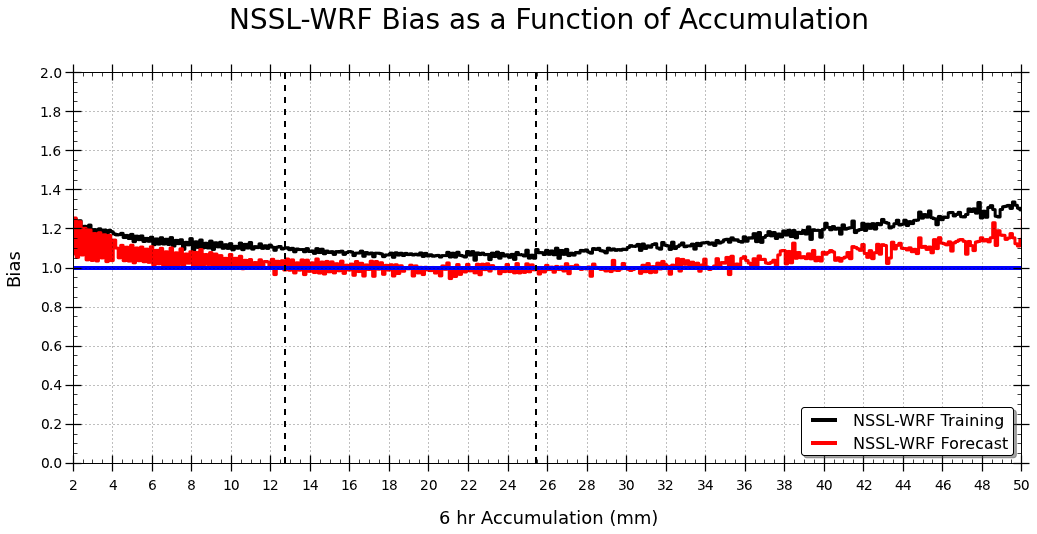
\includegraphics[width=\textwidth, height=\textheight, keepaspectratio]{%
    ./discussion/figs/nssl-wrf_bias}\\
    \caption{The NSSL-WRF forecast bias as a function of \mbox{6 hr} precipitation threshold.
    The black curve is the forecast bias calculated over the \mbox{36 month} training dataset.
    The rec curve is the forecast bias calculated over the \mbox{12 month} forecast dataset.
    The horizontal blue line depicts the line of perfect forecast bias.
    The vertical black dashed lines correspond to the \mbox{12.7 mm} threshold (left) and the \mbox{25.4 mm} threshold (right).}
    \label{nssl-wrf_bias}
\end{figure}


\clearpage
\begin{figure}[cc]
    \centering
    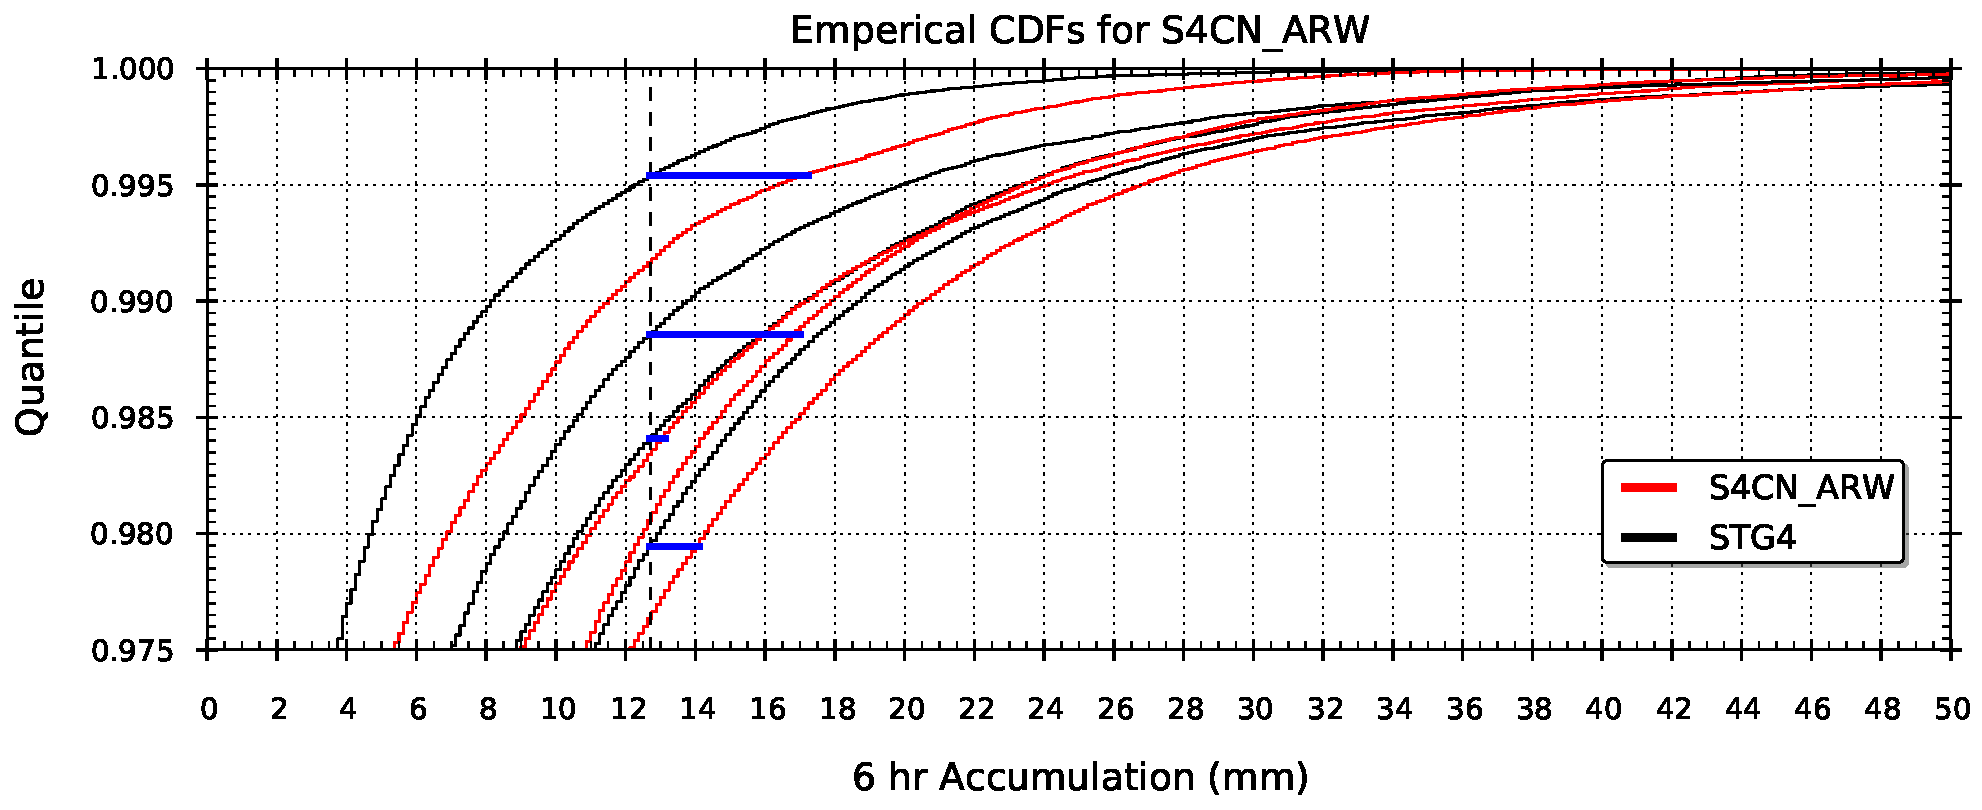
\includegraphics[width=\textwidth, height=\textheight, keepaspectratio]{%
    ./discussion/figs/ecdf_12mm_400km_s4cn_arw.pdf}\\
    \caption{The empirical cumulative distribution functions for the twenty simulations for both the Stage IV observations (black) and the CAPS SSEF WRF-ARW control member forecasts (red).
    The vertical black dashed line is the \mbox{25.4 mm} threshold.
    The horizontal blue dashed line is the connects the Stage IV quantile associated with the \mbox{12.7 mm} threshold to the equivalent quantile of the WRF-ARE control member.
    Where the blue line intersects the WRF-ARW control member empirical cumulative distribution function is the corresponding forecast threshold at which the ratio of points above to points below is equal to the Stage IV ratio of points above to points below the \mbox{12.7 mm} threshold.
    Note that the twenty simulations collapse into only four empirical cumulative distribution functions, depending on the dates selected.}
    \label{s4cn_arw_ecdf_12mm_400km}
\end{figure}


\begin{figure}[cc]
    \centering
    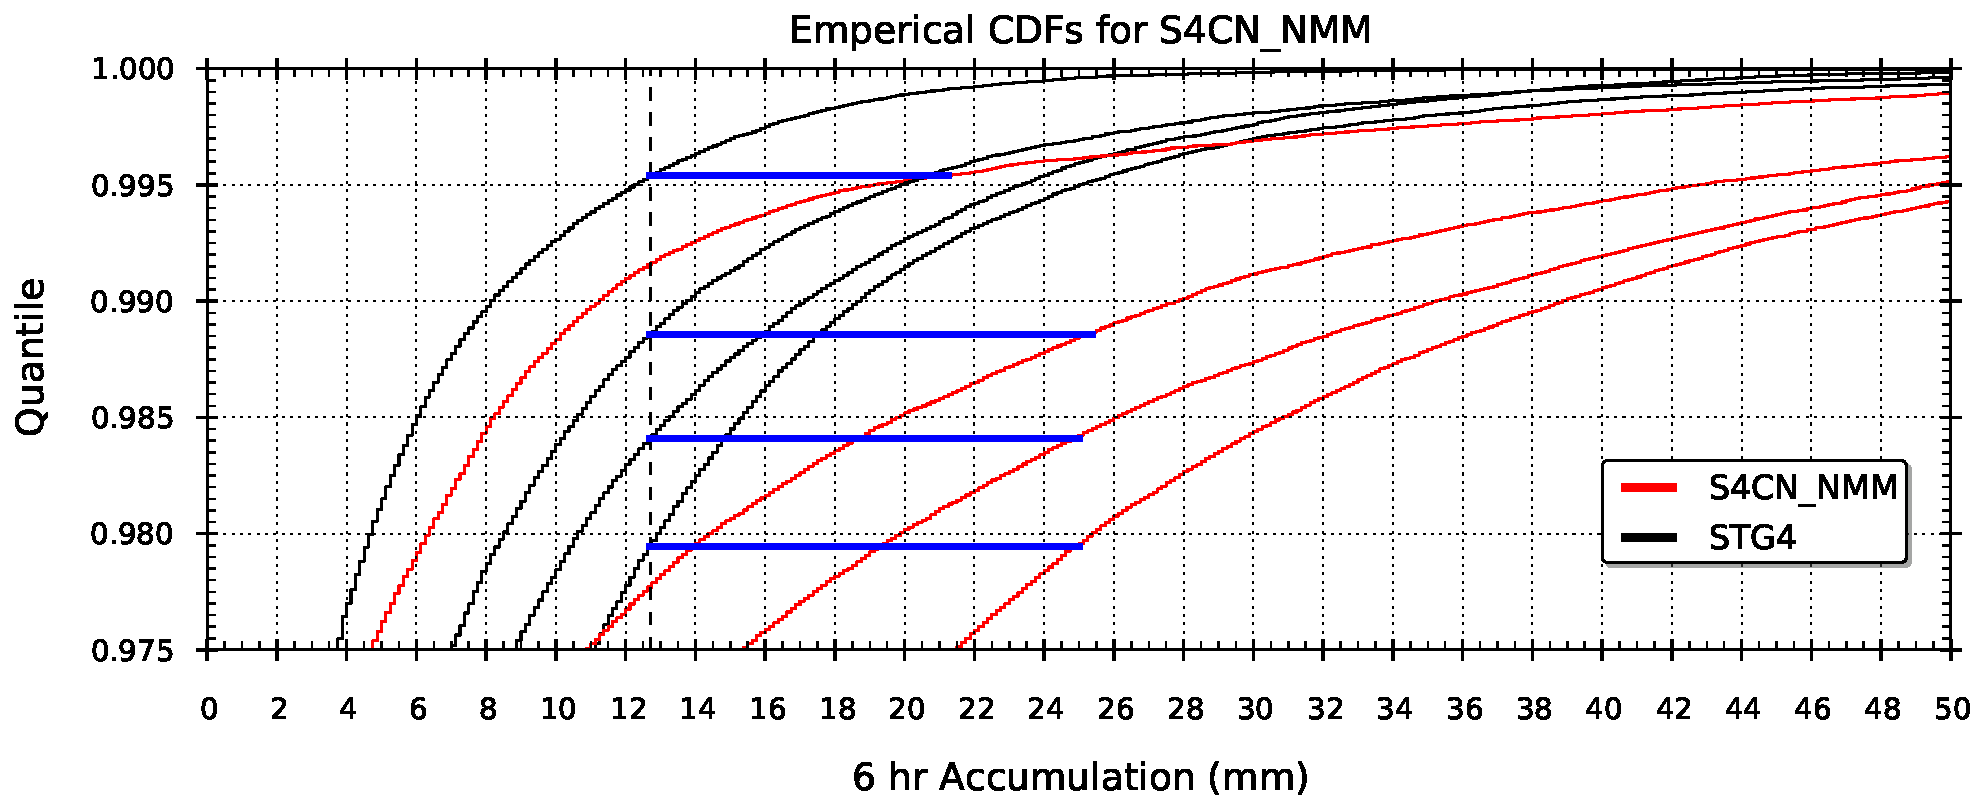
\includegraphics[width=\textwidth, height=\textheight, keepaspectratio]{%
    ./discussion/figs/ecdf_12mm_400km_s4cn_nmm.pdf}\\
    \caption{The same as in \mbox{Figure \ref{s4cn_arw_ecdf_12mm_400km}}, but for the CAPS SSEF WRF-NMM control member.
    Note the large disparity between the Stage IV empirical cumulative distribution function and the WRF-NMM control member.}
    \label{s4cn_nmm_ecdf_12mm_400km}
\end{figure}


\begin{oubibliography}
    \bibliographystyle{ametsoc}
    \bibliography{./bib/dissertation}
\end{oubibliography}


\makebackmatter
\end{document}
